\documentclass[slides,compress]{beamer}
\usepackage{graphicx,amsmath,hyperref}
\usepackage{verbatim}

\usepackage[normalem]{ulem}

\usetheme{default}
\useinnertheme{rectangles}

\title{\huge You can't get the staff - an electronic alternative...}
\subtitle{\large (an introduction to xia2)}

\author{Graeme Winter}
\institute{Diamond Light Source}
\date{CCP4 Study Weekend 2012}

\begin{document}

\setbeamertemplate{background}{
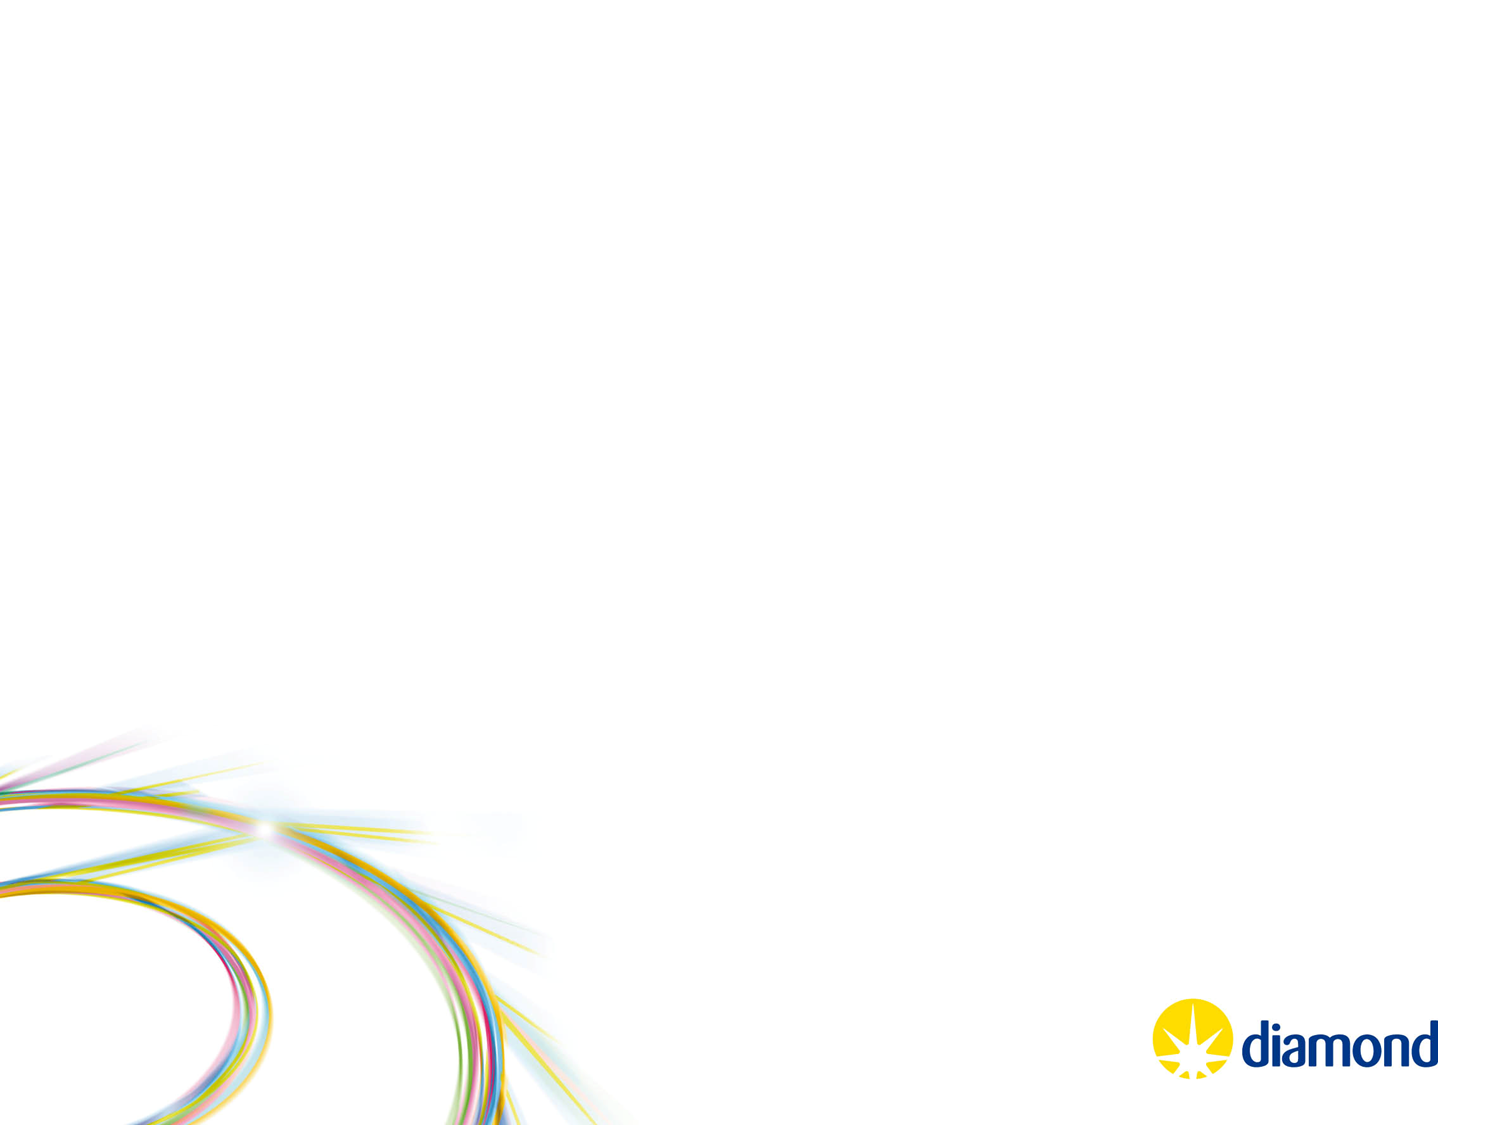
\includegraphics[width=\paperwidth,height=\paperheight]
{diamond-background.png}
}

\frame{\maketitle}

\frame{
\frametitle{Overview}
\begin{itemize}
\item{Background}
\item{What is xia2?}
\item{What does it do and how do I use it?}
\item{What decisions does it make?}
\item{Conclusions}
\end{itemize}
}

\section{Background}

\begin{frame}
\frametitle{Before we start...}
\begin{itemize}
\item{No 
MOSFLM\footnote{A.G.W. Leslie, Acta Cryst. (2006) D62, 48-57},
XDS\footnote{W. Kabsch, Acta Cryst. (2010) D66, 125-132}, 
SCALA\footnote{P. Evans, Acta Cryst. (2006) D62, 72-82}, 
CCP4\footnote{CCP4, Acta Cryst. (1994) D50, 760-763}
}
\item{$\rightarrow$ no xia2}
\item{No 
LABELIT\footnote{N.K. Sauter et al.
J. Appl. Cryst. (2004) 37, 399-409},
CCTBX\footnote{R.W. Grosse-Kunstleve et al.
J. Appl. Cryst. (2002) 35, 126-136},
POINTLESS\footnote{P. Evans, Acta Cryst. (2006) D62, 72-82}, 
etc.}
\item{$\rightarrow$ harder to write xia2, less reliable}
\end{itemize}
\end{frame}

\begin{frame}
\frametitle{Acknowledgements}
\begin{itemize}
\item{Andrew Leslie, Harry Powell, Phil Evans, Wolfgang Kabsch, Kay Diederichs,
Nick Sauter, Ralf Grosse-Kunstleve}
\item{Alun Ashton, Dave Stuart, Diamond beamline staff, Miroslav Papiz, 
Steve Prince, Colin Nave, xia2 users, providers of test data (esp. JCSG)}
\item{Funding from Diamond Light Source, BBSRC e-Science e-HTPX project, 
BioXHit}
\end{itemize}
\end{frame}

\begin{frame}
\frametitle{Background (2005)}
\begin{itemize}
\uncover<1->{
\item{Comprehensive, trusted software available}
\item{Background of strong publications (esp. CCP4 study weekends)}
\item{Massive advances in computing}
\item{New synchrotron for UK}
}
\uncover<2->{
\item{$\rightarrow$ a great time to develop automated data reduction}
}
\uncover<3->{
\item{\emph{Also told that this is impossible and a waste of time}}
}
\end{itemize}
\end{frame}

\section{What is xia2?}

\begin{frame}
\begin{center}
\Huge What is xia2?
\end{center}
\end{frame}

\begin{frame}
\frametitle{What is xia2?}
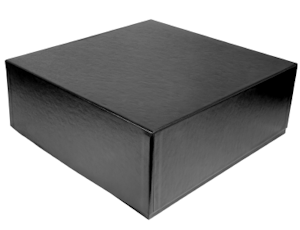
\includegraphics[scale=1]{figures/blackbox.png}
\end{frame}

\begin{frame}
\frametitle{What is xia2?}
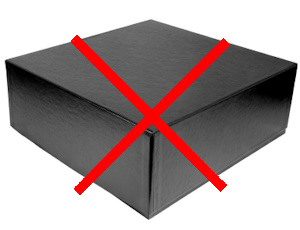
\includegraphics[scale=1]{figures/no-blackbox.png}
\end{frame}

\begin{frame}
\frametitle{What is xia2?}
{\large
\uncover<1->{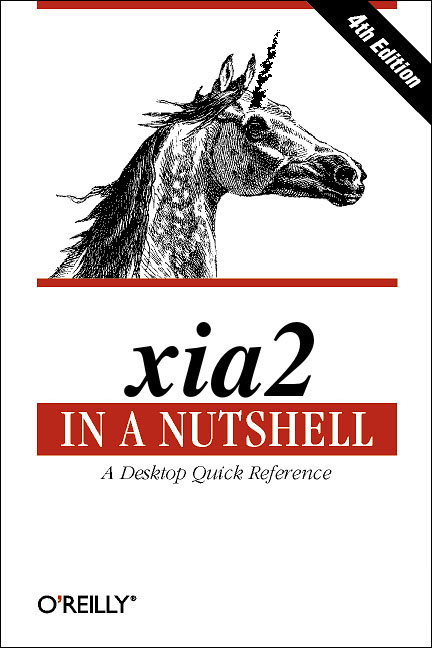
\includegraphics[scale=0.2]{figures/xia2-in-a-nutshell.jpg}}
\uncover<2->{
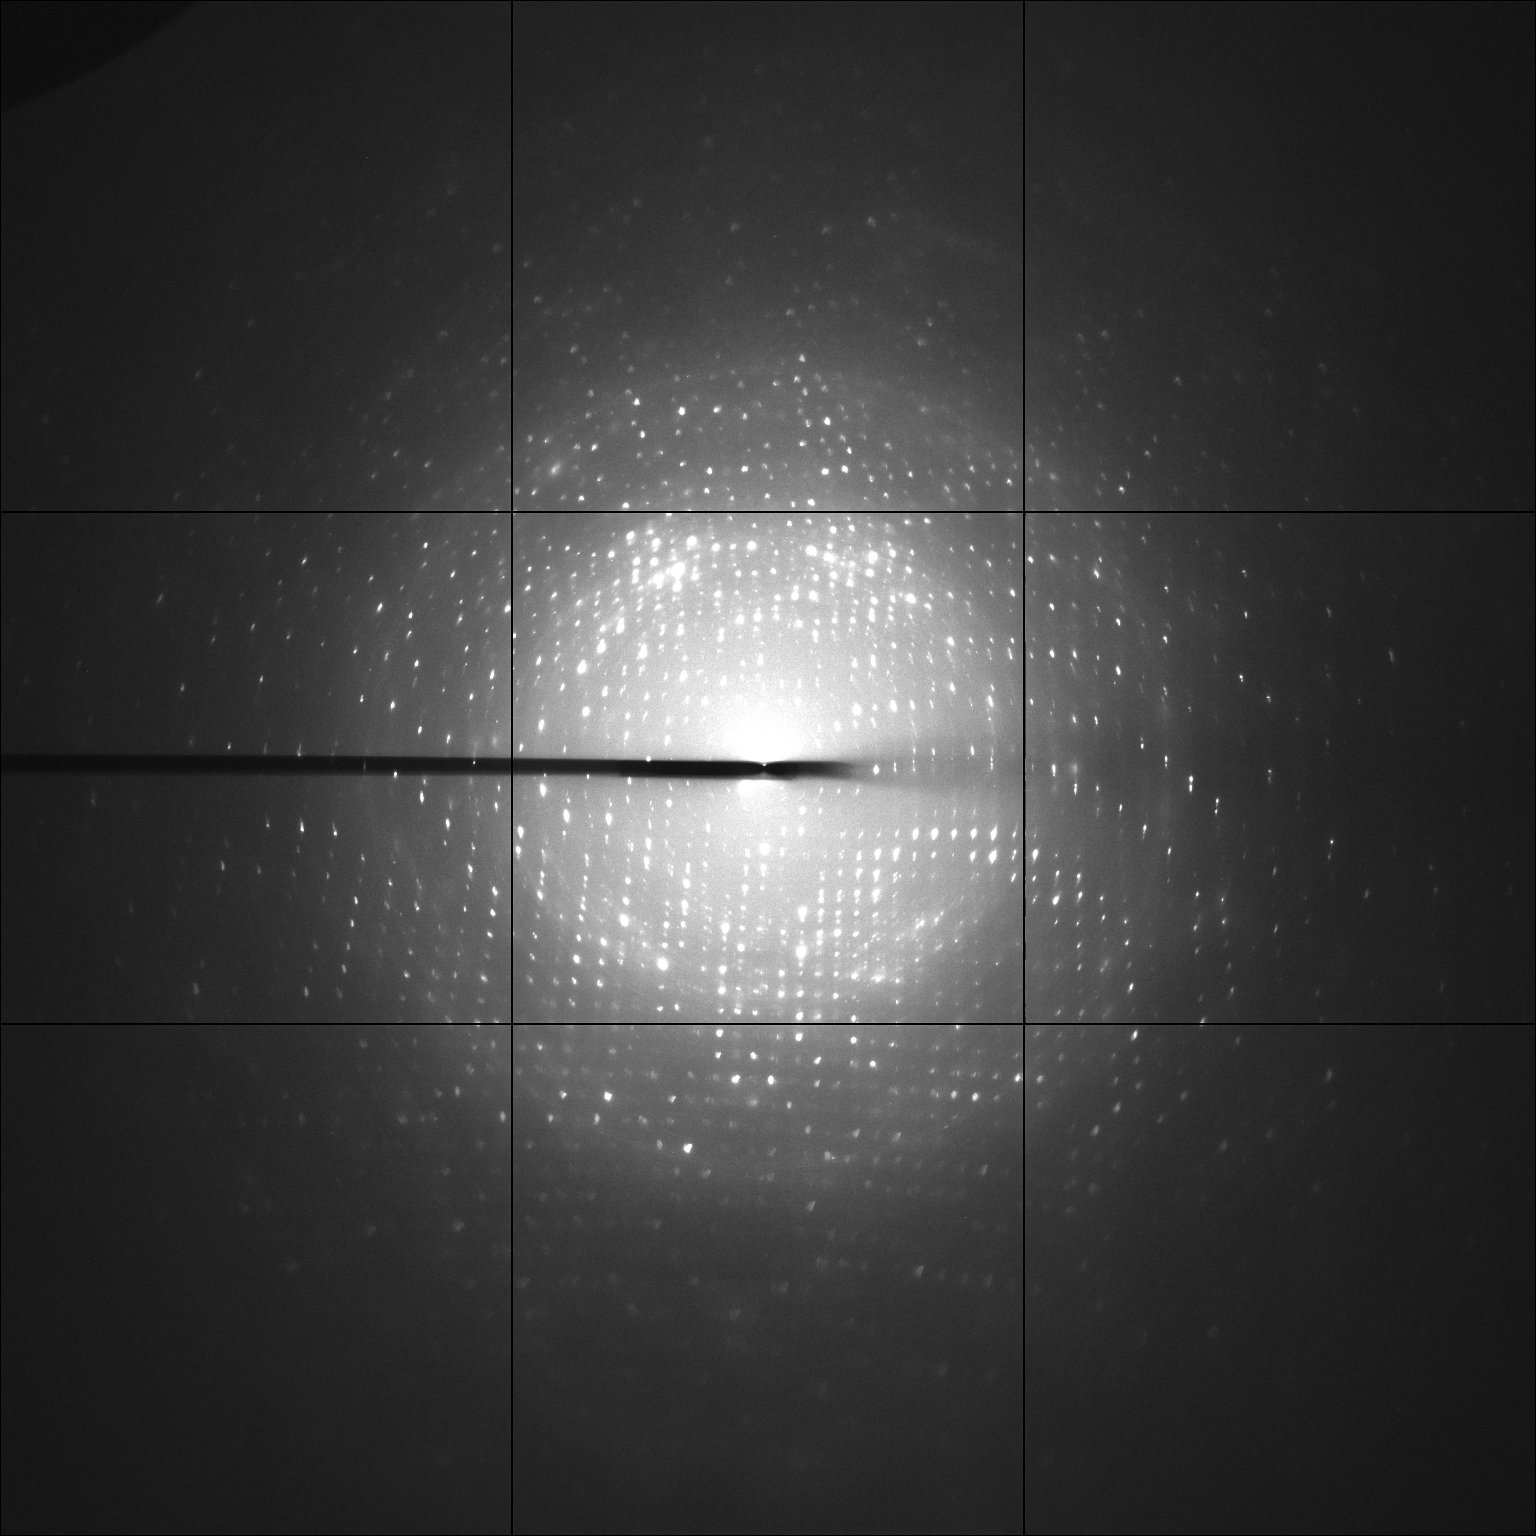
\includegraphics[scale=0.05]{figures/example-diffraction-image-small.jpg} 
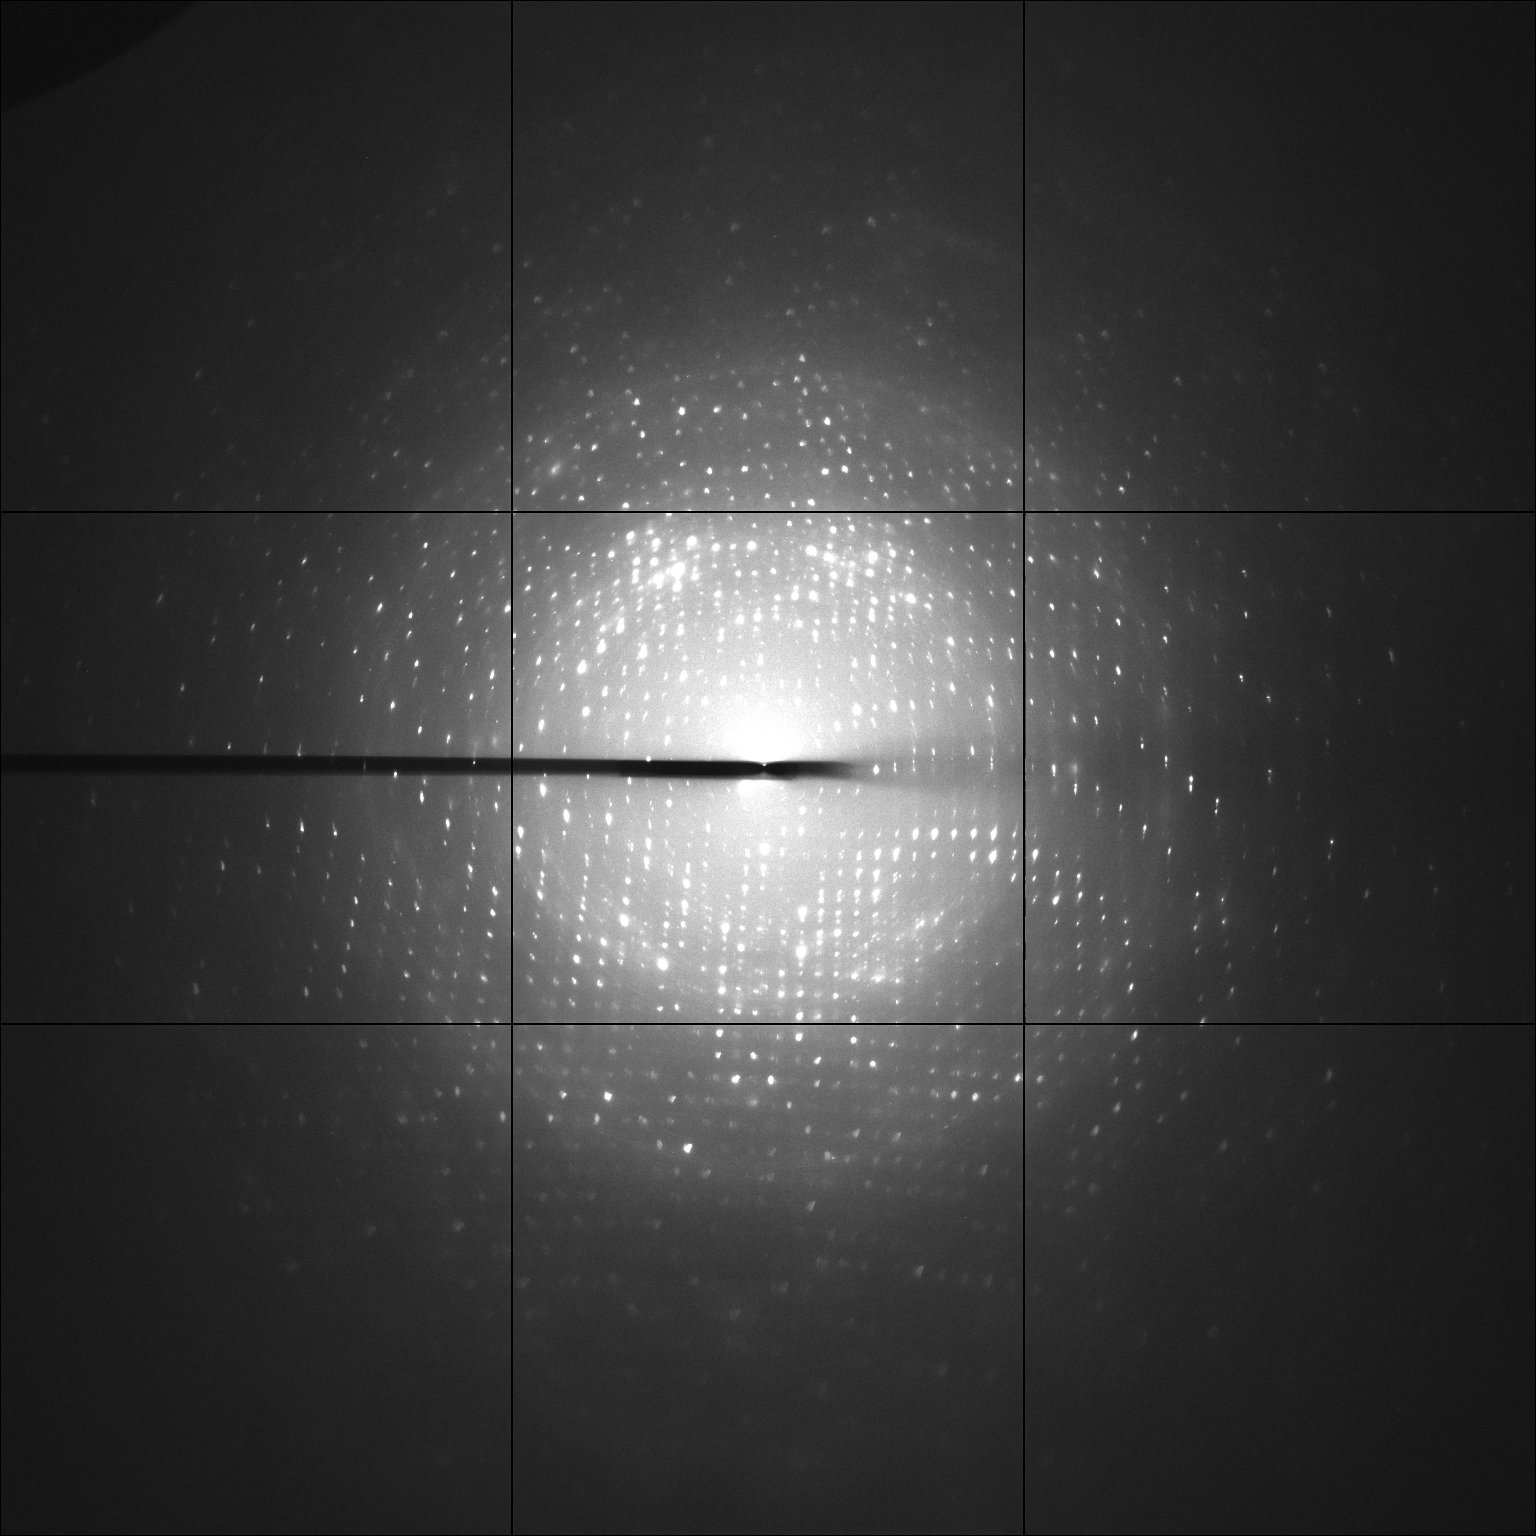
\includegraphics[scale=0.05]{figures/example-diffraction-image-small.jpg}
}
\uncover<3->{$\rightarrow H K L I \sigma_{I}$}
}
\end{frame}

\begin{frame}
\frametitle{What is xia2?}
\begin{itemize}
\uncover<1->{
\item{An \emph{expert} system to perform diffraction data processing 
and analysis on \emph{your} behalf using \emph{your} software}
}
\uncover<2->{
\item{A system which can correctly handle multi-pass, multi-wavelength data
sets}
}
\uncover<3->{
\item{\emph{Not} a data processing package}
}
\end{itemize}
\end{frame}

\begin{frame}
\frametitle{Why ``you can't get the staff?''}
\begin{columns}
\column{.5\textwidth}
\uncover<1->{
\begin{itemize}
\item{12 datasets / hour possible}
\item{Limited help}
\item{Human endurance}
\item{Intended xia2 as tool to delegate data processing to}
\end{itemize}
}
\column{.5\textwidth}
\uncover<2->{
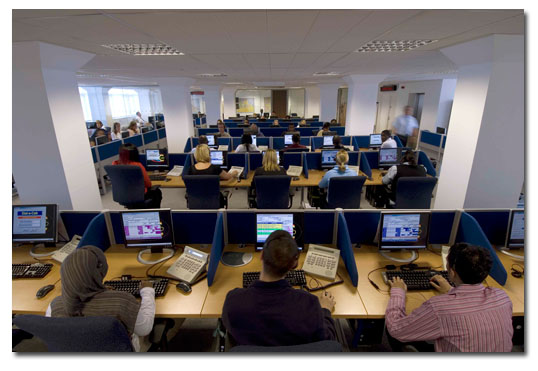
\includegraphics[scale=0.3]{figures/callcentre.jpg}
}
\end{columns}
\end{frame}

\begin{frame}
\frametitle{Why is this useful?}
\begin{itemize}
\item{Second opinion}
\item{Allows you to focus on problem cases}
\item{Help  busy / novice users}
\item{Provides access to other tools}
\item{Reproducible processing}
\end{itemize}
\end{frame}

\section{Using xia2}

\begin{frame}
\frametitle{Using xia2}
\begin{center}
\begin{tabular}{c}
{\huge
xia2 -2d /here/are/my/data
}\\
\\
{\huge \emph{- or -}} \\
\\
{\huge
xia2 -3d /here/are/my/data
}\\
\end{tabular}
\end{center}
\end{frame}

\begin{frame}
\frametitle{Command line}
\uncover<1-2>{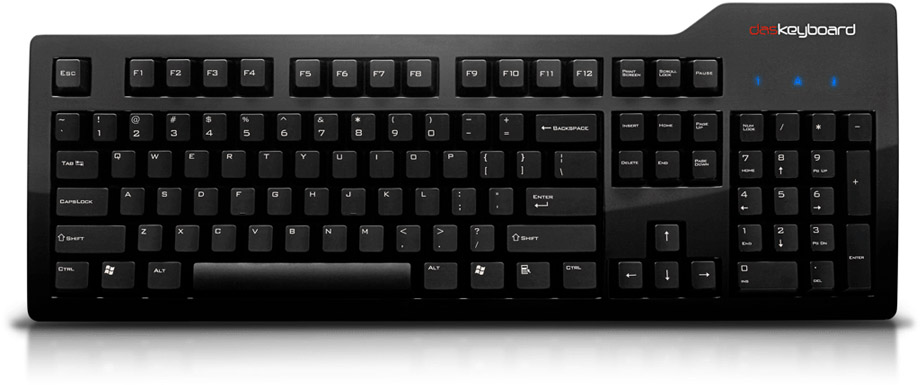
\includegraphics[scale=0.25]{figures/keyboard.jpg}}
\uncover<2-2>{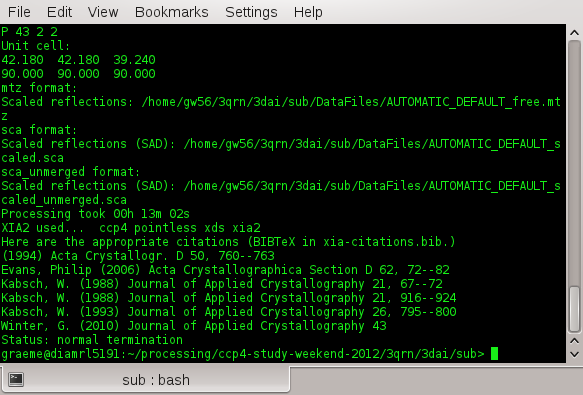
\includegraphics[scale=0.25]{figures/terminal.png}}
\end{frame}

\begin{frame}
\frametitle{Not GUI}
\begin{center}
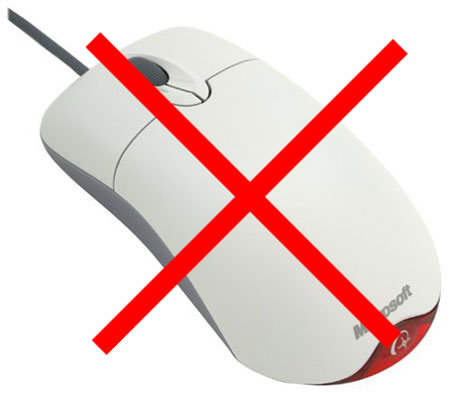
\includegraphics[scale=0.40]{figures/no-mouse.jpg}
\end{center}
\end{frame}

\begin{frame}
\frametitle{Options (1)}
\begin{itemize}
\item{-atom X - tell xia2 to separate anomalous pairs i.e. $I(+) \ne I(-)$ in 
scaling}
\item{-2d - tell xia2 to use MOSFLM and SCALA}
\item{-3d - tell xia2 to use XDS and XSCALE}
\item{-3dii - tell xia2 to use XDS and XSCALE, indexing with peaks found from
all images}
\end{itemize}
\end{frame}

\begin{frame}
\frametitle{How does it figure what to do?}
\begin{itemize}
\uncover<1->{\item{Read all of the image headers then}}
\uncover<2->{\item{Organise these into sweeps then}}
\uncover<3->{\item{Organise these into wavelengths then}}
\uncover<4->{\item{Assign all of these wavelengths to a crystal}}
\end{itemize}
\end{frame}

\begin{frame}
\frametitle{How does it figure what to do?}
\hspace{3cm}
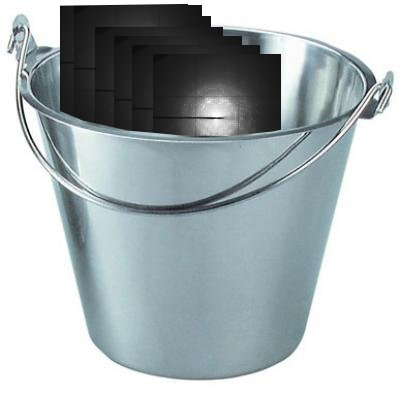
\includegraphics[scale=0.4]{figures/bucket-of-images.jpg}
\end{frame}

\begin{frame}
\frametitle{How does it figure what to do?}
\hspace{4cm}
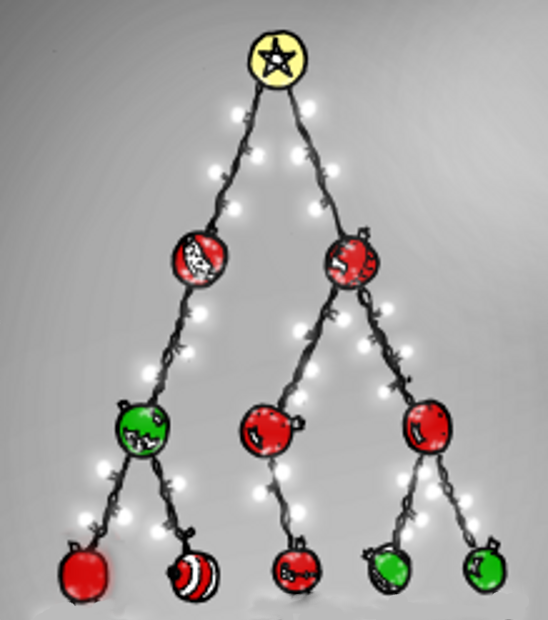
\includegraphics[scale=0.25]{figures/christmas-tree-nothing.png}
\end{frame}

\begin{frame}
\frametitle{How does it figure what to do?}
\hspace{4cm}
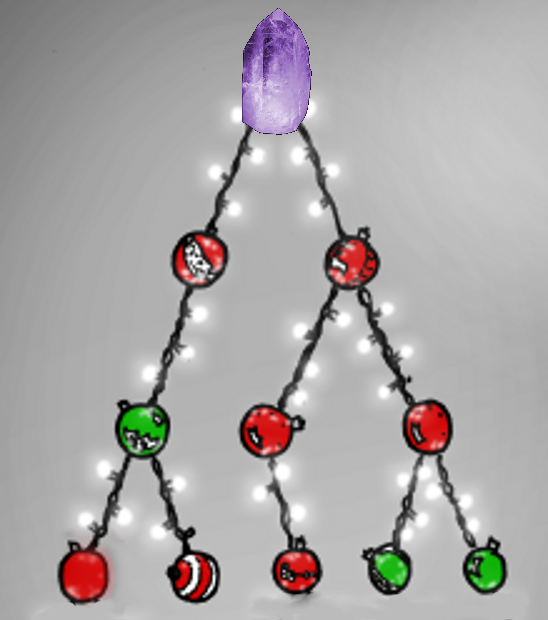
\includegraphics[scale=0.25]{figures/christmas-tree-nothing-crystal.png}
\end{frame}

\begin{frame}
\frametitle{How does it figure what to do?}
\hspace{4cm}
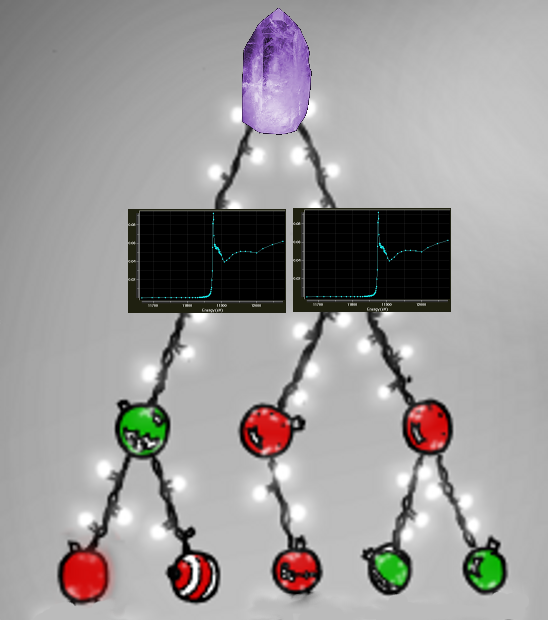
\includegraphics[scale=0.25]{figures/christmas-tree-nothing-wavelength.png}
\end{frame}

\begin{frame}
\frametitle{How does it figure what to do?}
\hspace{4cm}
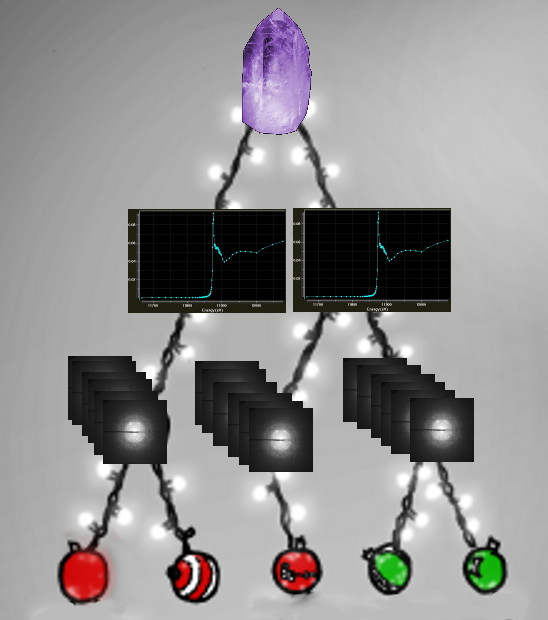
\includegraphics[scale=0.25]{figures/christmas-tree-nothing-sweep.png}
\end{frame}

\begin{frame}[fragile]
\frametitle{What the program sees (automatic.xinfo)}
{\small
\begin{verbatim}
BEGIN PROJECT AUTOMATIC
BEGIN CRYSTAL DEFAULT
BEGIN HA_INFO
ATOM Ba
END HA_INFO
BEGIN WAVELENGTH SAD
WAVELENGTH 0.979500
END WAVELENGTH SAD
BEGIN SWEEP SWEEP1
WAVELENGTH SAD
DIRECTORY /dls/i02/data/2011/mx1234-5
IMAGE K5_M1S3_3_001.img
START_END 1 450
END SWEEP SWEEP1
END CRYSTAL DEFAULT
END PROJECT AUTOMATIC
\end{verbatim}
}
\end{frame}

\begin{frame}
\frametitle{Understanding the experiment}
\begin{itemize}
\item{SWEEP: one ``scan'' - basic unit of indexing / integration}
\item{WAVELENGTH: container of SWEEPs}
\item{WAVELENGTH: all H K L observations merged}
\item{WAVELENGTH: CCP4 MTZ dataset}
\item{CRYSTAL: contains WAVELENGTHs}
\item{CRYSTAL: all data - basic unit of scaling}
\end{itemize}
\end{frame}

\begin{frame}
\frametitle{Example: 3QRN\footnote{J.P. Hall et al., Proc. Natl. Acad. Sci. USA 2011 108 (43) 17573-17574}}
\begin{itemize}
\item{Data recorded at Diamond I02}
\item{DNA / ligand complex}
\item{Demonstrates:
\begin{itemize}
\item{Radiation damage}
\item{Heavy atom}
\item{Resolution limits}
\end{itemize}
}
\item{Better sample used for deposition}
\end{itemize}
\end{frame}

\begin{frame}
\frametitle{Example: data}
\begin{center}
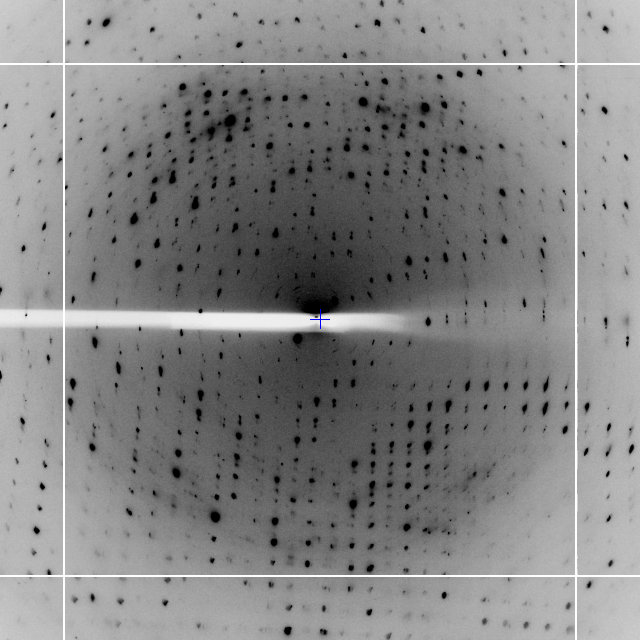
\includegraphics[scale=0.35]{figures/3qrn-diffraction.png}
\end{center}
\end{frame}

\begin{frame}
\frametitle{Example command line}
{ \huge
xia2 -3d -atom Ba /dls/i02/data/...
}
\end{frame}

\begin{frame}
\frametitle{Example results}
\begin{tabular}{lccc}
High resolution limit      &       \color{red}{1.25} &    6.45 &   1.25\\
Low resolution limit       &                18.85  & 18.85  &  1.27\\
Completeness               &                95.2   & 60.1  &  70.2\\
Multiplicity               &               12.2    & 8.4   &  4.8\\
I/sigma                    &               12.3    & 18.5   &  2.6\\
Rmerge                     &             \color{red}{0.113}  & 
\color{red}{0.096} &  0.564\\
Rmeas(I)                   &             0.129  & 0.118 &  0.633\\
Rmeas(I+/-)                &             0.121  & 0.105 &  0.679\\
Rpim(I)                    &             0.034  & 0.038 &  0.267\\
Rpim(I+/-)                 &             0.043  & 0.041 &  0.368\\
Wilson B factor            &            12.131& & \\
Anomalous completeness     &            93.3  &  52.6  &  58.0\\
Anomalous multiplicity     &           6.4    & 5.0  &   2.0\\
Anomalous correlation      &            0.544 &  0.791 & -0.297\\
Anomalous slope            &      1.085 &  0.000 &  0.000\\
Total observations         &       118588 & 529  &   1634\\
Total unique               &         9749  &  63 &     337\\
\end{tabular}
\end{frame}

\begin{frame}
\frametitle{Development option - using AIMLESS}
{ \huge
xia2 -3da ...
}
\end{frame}

\begin{frame}
\frametitle{LogFiles/*aimless.log}
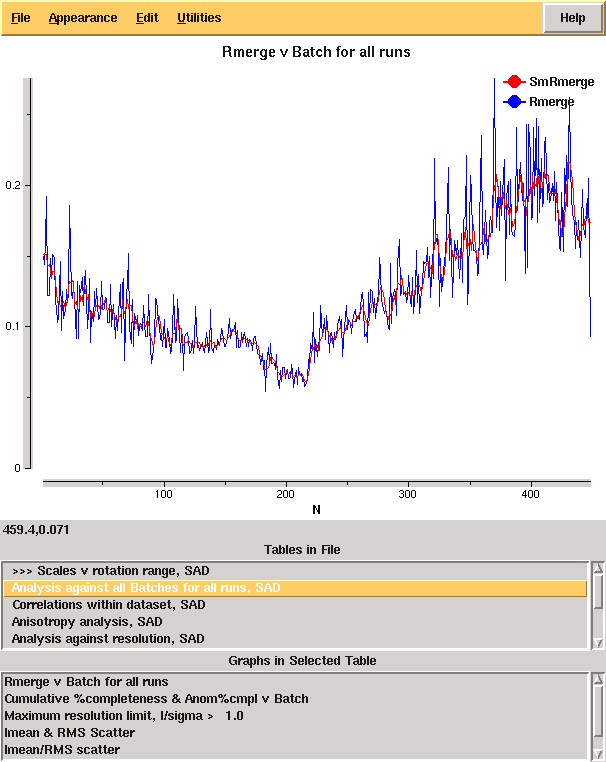
\includegraphics[scale=0.25]{figures/3qrn-all-rmerge-aimless.png}
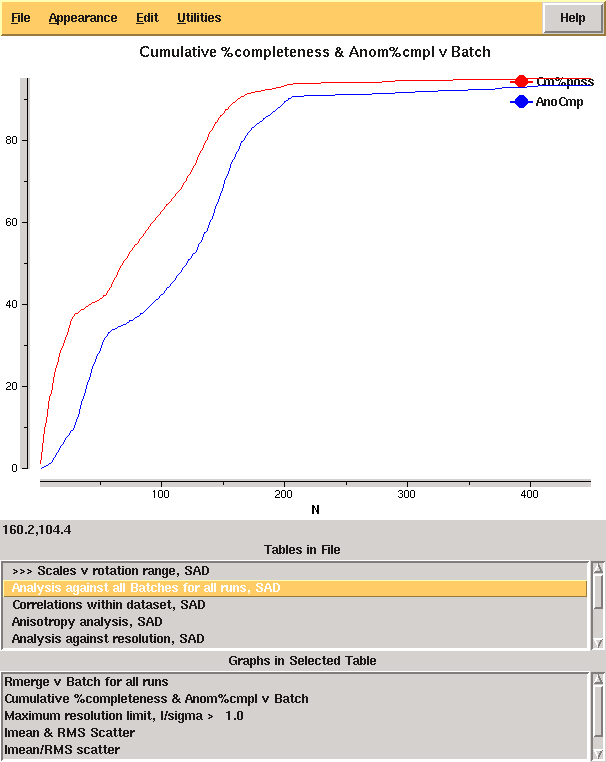
\includegraphics[scale=0.25]{figures/3qrn-all-complete-aimless.png}
\end{frame}

\begin{frame}
\frametitle{What to do next?}
\begin{itemize}
\item{Edit automatic.xinfo}
\item{Only process first 200 frames}
\end{itemize}
\end{frame}

\begin{frame}[fragile]
\frametitle{Modify automatic.xinfo $\rightarrow$ modified.xinfo}
{\small
\begin{verbatim}
BEGIN PROJECT AUTOMATIC
BEGIN CRYSTAL DEFAULT
BEGIN HA_INFO
ATOM Ba
END HA_INFO
BEGIN WAVELENGTH SAD
WAVELENGTH 0.979500
END WAVELENGTH SAD
BEGIN SWEEP SWEEP1
WAVELENGTH SAD
DIRECTORY /dls/i02/data/2011/mx1234-5
IMAGE K5_M1S3_3_001.img
START_END 1 200 ! THIS WAS 450
END SWEEP SWEEP1
END CRYSTAL DEFAULT
END PROJECT AUTOMATIC
\end{verbatim}
}
\end{frame}

\begin{frame}
\frametitle{Running again}
\begin{center}
\huge xia2 -3d -xinfo modified.xinfo
\end{center}
\end{frame}

\begin{frame}
\frametitle{Example results II}
\begin{tabular}{lccc}
High resolution limit         &         1.22 &  6.34 &  1.22 \\
Low resolution limit          &        19.62 & 19.62 &  1.24 \\
Completeness                  &         86.9 &  49.1 &  37.8 \\
Multiplicity                  &        5.3  &  4.9   & 1.7 \\
I/sigma                       &        20.1 &  37.0  &  2.3 \\
Rmerge                        &       0.036 & 0.020  &0.355 \\
Rmeas(I)                      &       0.060 & 0.038  &0.448 \\
Rmeas(I+/-)                   &       0.043 & 0.023  &0.491 \\
Rpim(I)                       &       0.023 & 0.014  &0.297 \\
Rpim(I+/-)                    &       0.022 & 0.011  &0.339 \\
Wilson B factor               &       10.70& \\
Anomalous completeness        &        77.7  & 41.0  & 18.3 \\
Anomalous multiplicity        &         2.7  &  3.5  &  0.5 \\
Anomalous correlation         &        0.779 & 0.931 & 0.000 \\
Anomalous slope               &       1.553  &0.000 & 0.000 \\
Total observations            &       50875  &272   & 342 \\
Total unique                  &       9552   &55    & 199 \\
\end{tabular}
\end{frame}

\begin{frame}
\frametitle{Resolution: much more in Lunchtime Bytes}
\begin{itemize}
\item{Data incomplete at high resolution}
\item{Add RESOLUTION to xinfo file (in either SWEEP or WAVELENGTH}
\item{Add -resolution to the command line}
\end{itemize}
\end{frame}

\begin{frame}
\frametitle{Output}
\begin{itemize}
\item{xia2.txt: everything you should read - including program citations}
\item{xia2-debug.txt: everything you probably shouldn't}
\item{LogFiles: you should look at these}
\item{DataFiles: MTZ + erzatz scalepack}
\end{itemize}
\end{frame}

\begin{frame}[fragile]
\frametitle{Output}
{\small
\begin{verbatim}
------------------- Autoindexing SWEEP1 --------------------
All possible indexing solutions:
tP  57.60  57.60 149.51  90.00  90.00  90.00
oC  81.45  81.46 149.51  90.00  90.00  90.00
oP  57.59  57.60 149.50  90.00  90.00  90.00
mC  81.46  81.45 149.50  90.00  89.95  90.00
mP  57.60  57.59 149.53  90.00  89.93  90.00
aP  57.59  57.61 149.52  89.93  89.99  89.99
Indexing solution:
tP  57.60  57.60 149.51  90.00  90.00  90.00
\end{verbatim}
}
\end{frame}

\begin{frame}[fragile]
\frametitle{Output}
{\small
\begin{verbatim}
-------------------- Integrating SWEEP1 --------------------
Processed batches 1 to 450
Weighted RMSD: 0.26 (0.09)
Integration status per image (60/record):
ooooooooooooooooooooooooooooooooooo.oooooooooooooooooooooooo
ooooooooooooooooooooooo.ooooooooooooooooooo.ooooooo.oooooooo
ooo.o.ooooooo.oooooooooooooooooooooooooooooooooooooooooooooo
oooooooooooooooooooooooooooooooooooooooooooooooooooooooooooo
oooooooooooooooooooo.ooooooooooooooooooooooooooooooooooooooo
ooooooooooooooooooooooooooooooooooooooooooooooooooo.oooooooo
ooooooooo.oooooooooo..ooo.oooooooooooooooooooo.ooooooooooooo
oooooooooooooooooooo.oooooooo.
"o" => good        "%" => ok        "!" => bad rmsd
"O" => overloaded  "#" => many bad  "." => blank
"@" => abandoned
Mosaic spread: 0.140 < 0.189 < 0.290
\end{verbatim}
}
\end{frame}

\begin{frame}
\frametitle{Options (2)}
\begin{itemize}
\item{-xinfo modified.xinfo - use specific input file}
\item{-image /path/to/an/image.img - process specific scan}
\item{-spacegroup spacegroup\_name - set the spacegroup, e.g. P21}
\item{-cell a,b,c,$\alpha$,$\beta$,$\gamma$ - set the cell constants} 
\item{-small\_molecule - don't run things like TRUNCATE}
\end{itemize}
\end{frame}

\section{What did it do?}

\begin{frame}
\begin{center}
\Huge What did it do? and why?
\end{center}
\end{frame}

\begin{frame}
\frametitle{Indexing}
\begin{itemize}
\item{Initial indexing with LABELIT from 3 images\footnote{This is \emph{not}
good for small molecule data}}
\item{Refine results with XDS indexing}
\item{Use data based on general analysis @ 0, 45, 90 degrees}
\end{itemize}
\end{frame}

\begin{frame}
\frametitle{Integration}
\begin{itemize}
\item{Integrate with lattice constraints applied}
\item{Integrate to corners of detector}
\item{If good reason, repeat integration e.g. with results of postrefinement}
\item{Perform postrefinement in P1, assumed lattice - may reject lattice,
feed back to indexing}
\item{At the end of this we have LATTICE}
\item{If XDS, includes iterative elimination of outliers in CORRECT step}
\end{itemize}
\end{frame}

\begin{frame}
\frametitle{Scaling}
\begin{itemize}
\item{Compare results of pointless with remaining allowed lattices:
\begin{itemize}
\item{If agree, proceed}
\item{If lattice not allowed, consider next solution}
\item{If solution lower symmetry than lattice, reject and return to indexing}
\end{itemize}
}
\item{Ensure conclusions consistent}
\item{Now have corrrect LAUE GROUP}
\item{Ensure consistent setting / origin choice}
\item{Place data into data collection order}
\item{Analyse absences to decide likely SPACE GROUPs}
\item{Decide scaling model\footnote{For XDS use not corrections in CORRECT,
apply all corrections in XSCALE}}
\end{itemize}
\end{frame}

\begin{frame}
\frametitle{Merging and analysis}
\begin{itemize}
\uncover<1->{
\item{If using XDS for integration and XSCALE for scaling, data still merged
with SCALA / AIMLESS}
\item{Resolution limits calculated from the intensities, not program output}
\item{``Downstream'' analysis (e.g. TRUNCATE and SFCHECK) identical}
}
\uncover<2->{\item{Working on scaling data direct from XDS with AIMLESS}}
\end{itemize}
\end{frame}

\section{What decisions were made?}

\begin{frame}
\begin{center}
\Huge Decision making
\end{center}
\end{frame}

\begin{frame}[fragile]
\frametitle{Decisions: Indexing - LABELIT}
{\small
\begin{verbatim}
Solution  Metric fit  rmsd  #spots  crystal_system   unit_cell 
:)   9     0.2097 dg 0.327    533    tetragonal tP   42.32  42.32  39.28  ...
:)   8     0.2097 dg 0.364    541  orthorhombic oP   39.29  42.28  42.33  ...
:)   7     0.2097 dg 0.300    519    monoclinic mP   39.26  42.32  42.32  ...
:)   6     0.1950 dg 0.299    523    monoclinic mP   39.26  42.33  42.31  ...
:)   5     0.1307 dg 0.411    523  orthorhombic oC   59.71  59.91  39.31  ...
:)   4     0.1307 dg 0.412    524    monoclinic mC   59.91  59.71  39.31  ...
:)   3     0.0937 dg 0.429    524    monoclinic mC   59.71  59.91  39.30  ...
:)   2     0.1010 dg 0.298    512    monoclinic mP   42.27  39.31  42.32  ...
:)   1     0.0000 dg 0.291    509     triclinic aP   39.31  42.26  42.32  ...
\end{verbatim}
}
\end{frame}

\begin{frame}[fragile]
\frametitle{Decisions: Indexing - IDXREF}
{\small
\begin{verbatim}
 *  31        aP          0.0      39.1   42.1   42.1  90.0  90.0  89.9
 *  44        aP          0.1      39.1   42.1   42.1  90.0  90.0  90.1
 *  34        mP          0.7      39.1   42.1   42.1  90.0  90.1  90.0
 *  20        mC          0.7      59.6   59.6   39.1  90.1  90.1  90.0
 *  33        mP          0.8      39.1   42.1   42.1  90.0  90.1  90.0
 *  25        mC          0.9      59.6   59.6   39.1  89.9  90.1  90.0
 *  35        mP          1.7      42.1   39.1   42.1  90.0  90.0  90.1
 *  23        oC          1.7      59.6   59.6   39.1  89.9  90.1  90.0
 *  32        oP          1.8      39.1   42.1   42.1  90.0  90.0  90.1
 *  21        tP          1.9      42.1   42.1   39.1  90.0  90.1  90.0
    10        mC         79.5      57.5   57.4   42.1  90.0  90.0  94.2
    13        oC         79.9      57.4   57.5   42.1  90.0  90.0  85.8
    14        mC         79.9      57.4   57.5   42.1  90.0  90.0  85.8
\end{verbatim}
}
\end{frame}

\begin{frame}
\frametitle{Decisions: Testing lattice choice}
\begin{itemize}
\item{Perform postrefinement (MOSFLM and XDS) in P1 and putative lattice}
\item{Compare R.M.S. deviation of observed / predicted centres}
\item{Results comparable $\rightarrow$ lattice probably OK}
\item{Results worse with lattice constraints $\rightarrow$ lattice probably
wrong}
\end{itemize}
\end{frame}

\begin{frame}[fragile]
\frametitle{Decisions: Testing lattice choice 1}
{\small
\begin{verbatim}
 REFINED PARAMETERS:  DISTANCE BEAM ORIENTATION CELL AXIS                   
 USING   27389 INDEXED SPOTS
 STANDARD DEVIATION OF SPOT    POSITION (PIXELS)     1.28
 STANDARD DEVIATION OF SPINDLE POSITION (DEGREES)    0.23
...
 UNIT CELL PARAMETERS     42.180    42.183    39.236  90.002  89.989  89.986
 E.S.D. OF CELL PARAMETERS  1.8E-02 4.3E-02 1.5E-02 1.4E-02 1.0E-02 2.9E-02
 SPACE GROUP NUMBER      1
\end{verbatim}
}
\end{frame}

\begin{frame}[fragile]
\frametitle{Decisions: Testing lattice choice 2}
{\small
\begin{verbatim}
 REFINED PARAMETERS:  DISTANCE BEAM ORIENTATION CELL AXIS                   
 USING   27378 INDEXED SPOTS
 STANDARD DEVIATION OF SPOT    POSITION (PIXELS)     1.29
 STANDARD DEVIATION OF SPINDLE POSITION (DEGREES)    0.23
...
 UNIT CELL PARAMETERS     42.187    42.187    39.242  90.000  90.000  90.000
 E.S.D. OF CELL PARAMETERS  1.6E-02 1.6E-02 1.2E-02 0.0E+00 0.0E+00 0.0E+00
 SPACE GROUP NUMBER     75
\end{verbatim}
}
\end{frame}

\begin{frame}
\frametitle{Decisions: Lattice observations}
\begin{itemize}
\item{Selecting lattice from indexing safe, as tested and challenged}
\item{However strong argument for performing all processing in P1:
\begin{itemize}
\item{Processing only performed once}
\item{Incorrect constraints cannot break things}
\item{Results generally comparable}
\end{itemize}
}
\item{This is on the to-do list...}
\end{itemize}
\end{frame}

\begin{frame}
\frametitle{Resolution limits - default criteria}
\begin{itemize}
\item{Merged $\frac{I}{\sigma_I} > 2$}
\item{Unerged $\frac{I}{\sigma_I} > 1$}
\item{Control with -misigma, -isigma}
\end{itemize}
\end{frame}

\begin{frame}
\frametitle{Resolution limits - why unmerged $\frac{I}{\sigma_I} > 1$?}
\hspace{6cm}
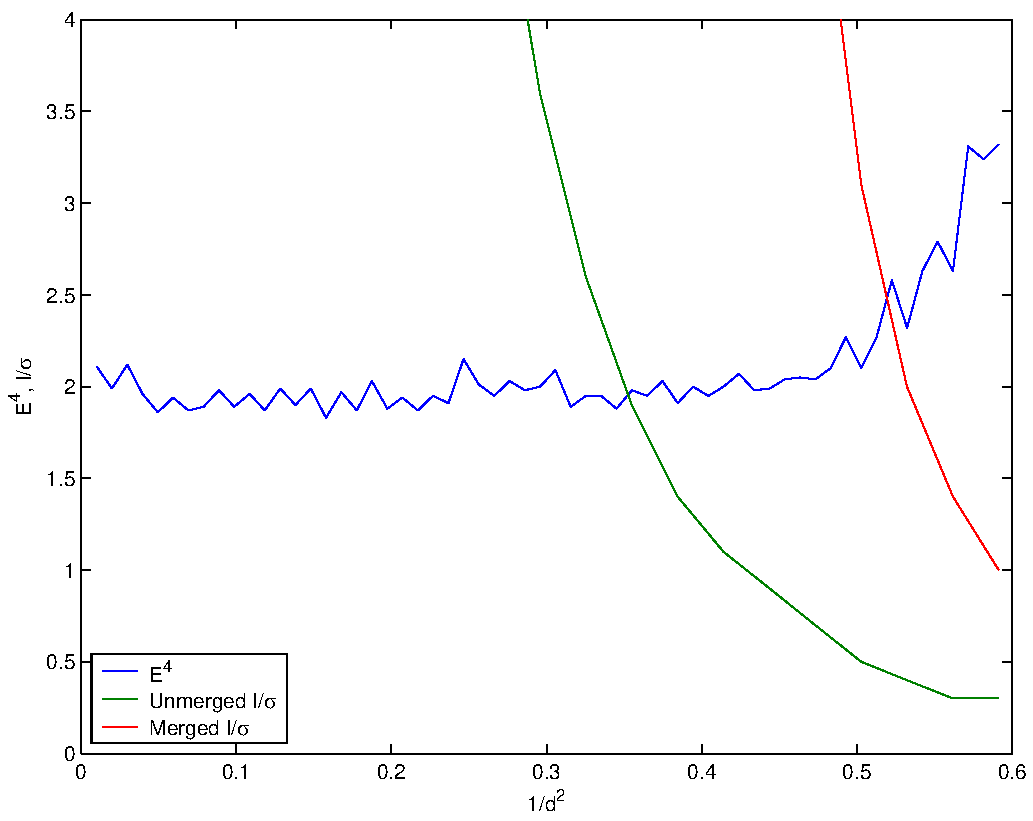
\includegraphics[scale=0.5]{figures/plat-13A-z4.pdf}
\footnote{90-fold multiplicity data from Ed Mitchell @ ESRF}
\end{frame}

\section{Comments}

\begin{frame}
\frametitle{Which options work best?}
\begin{itemize}
\uncover<1->{
\item{It depends ...}
\item{... try for yourself!}
}
\uncover<2->{
\item{Sometimes -2d (MOSFLM / SCALA) works better, sometimes -3d (XDS etc.)}
}
\uncover<3->{
\item{Run both - compare results, make up your own mind}
}
\uncover<4->{
\item{Hint for small molecule: -3dii -small\_molecule}
}
\uncover<5->{
\item{-3d often works better for very fine $\phi$ sliced Pilatus data}
}
\end{itemize}
\end{frame}

\section{Conclusions}

\begin{frame}
\frametitle{Conclusions}
\begin{itemize}
\item{System available which can reduce your data on your behalf}
\item{Relies on your software: MOSFLM / LABELIT / CCP4 / XDS}
\item{Handles complex strategies so use them}
\item{Works on Windows / OS X / Linux / laptop / workstation / cluster}
\end{itemize}
\end{frame}

\begin{frame}
\frametitle{Conclusions}
\begin{itemize}
\item{Best way to learn data reduction is to teach it}
\item{Computer is very dim but diligent pupil}
\item{Have a go yourself, or feel free to contribute to xia2}
\end{itemize}
\end{frame}

\begin{frame}
\frametitle{Getting xia2}
\begin{itemize}
\item{Blog: xia2.blogspot.com}
\item{Code: xia2.sf.net}
\item{List: xia2-list@lists.sourceforge.net}
\end{itemize}
\end{frame}

\begin{frame}
\begin{center}
\Huge Thank you for your attention
\end{center}
\end{frame}

\begin{frame}
\begin{center}
\Huge Spare slides
\end{center}
\end{frame}

\begin{frame}
\frametitle{Indexing}
\hspace{3cm}
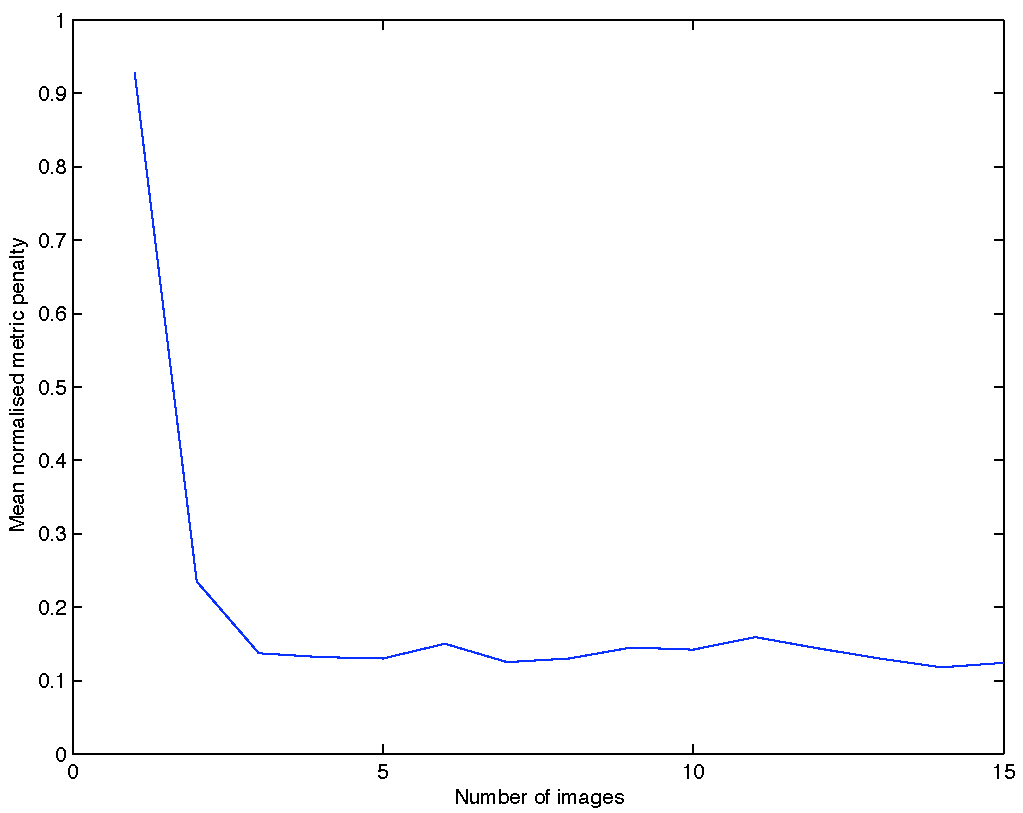
\includegraphics[scale=0.5]{figures/no_images.pdf}
\end{frame}

\begin{frame}
\frametitle{Indexing}
\hspace{3cm}
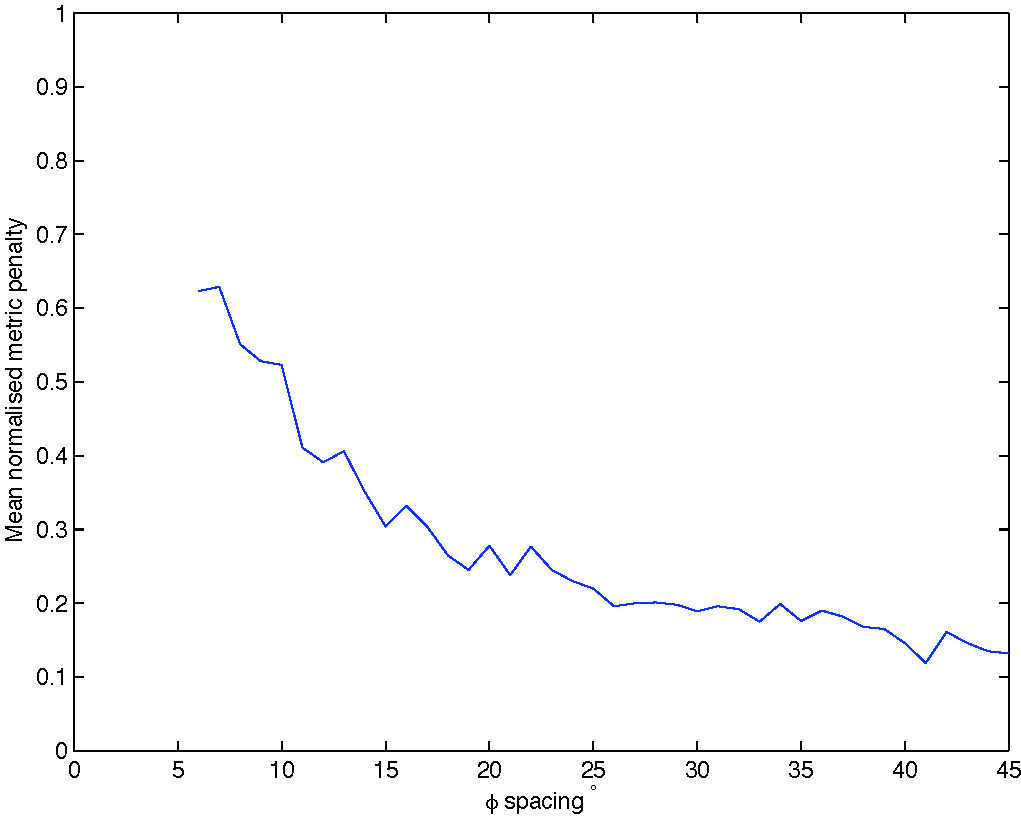
\includegraphics[scale=0.5]{figures/phi_spacing_45a.pdf}
\end{frame}

\begin{frame}
\frametitle{Indexing}
\hspace{3cm}
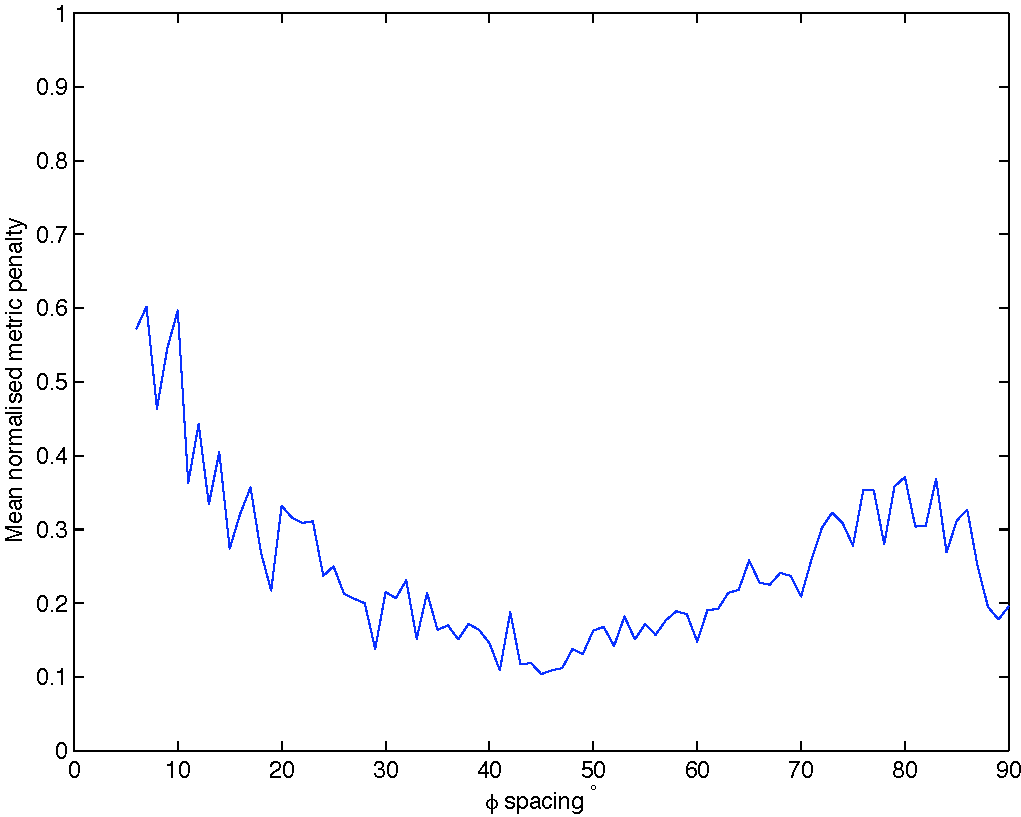
\includegraphics[scale=0.5]{figures/phi_spacing_90a.pdf}
\end{frame}

\begin{frame}
\frametitle{Indexing}
\hspace{6cm}
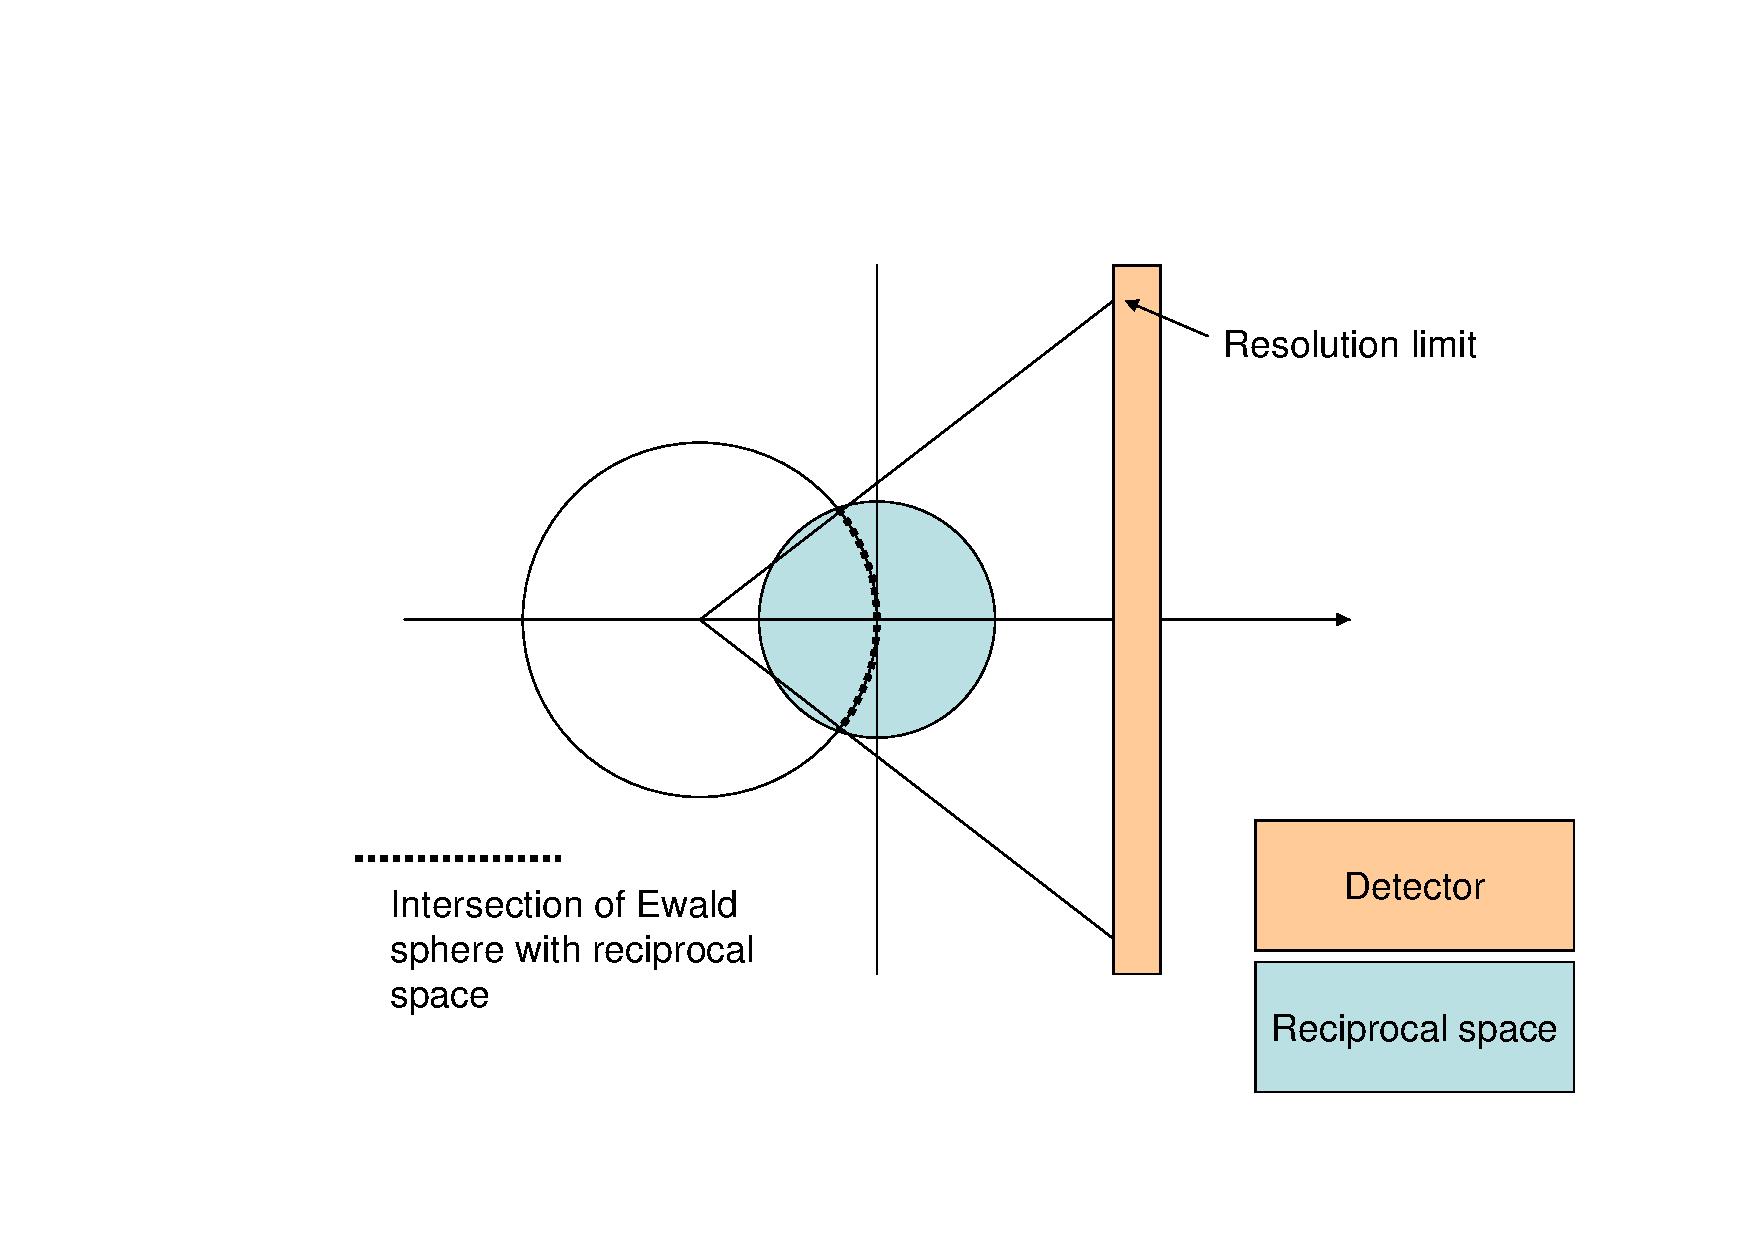
\includegraphics[scale=0.5]{figures/EwaldExplain.pdf}
\end{frame}

\begin{frame}
\frametitle{Indexing}
\hspace{6cm}
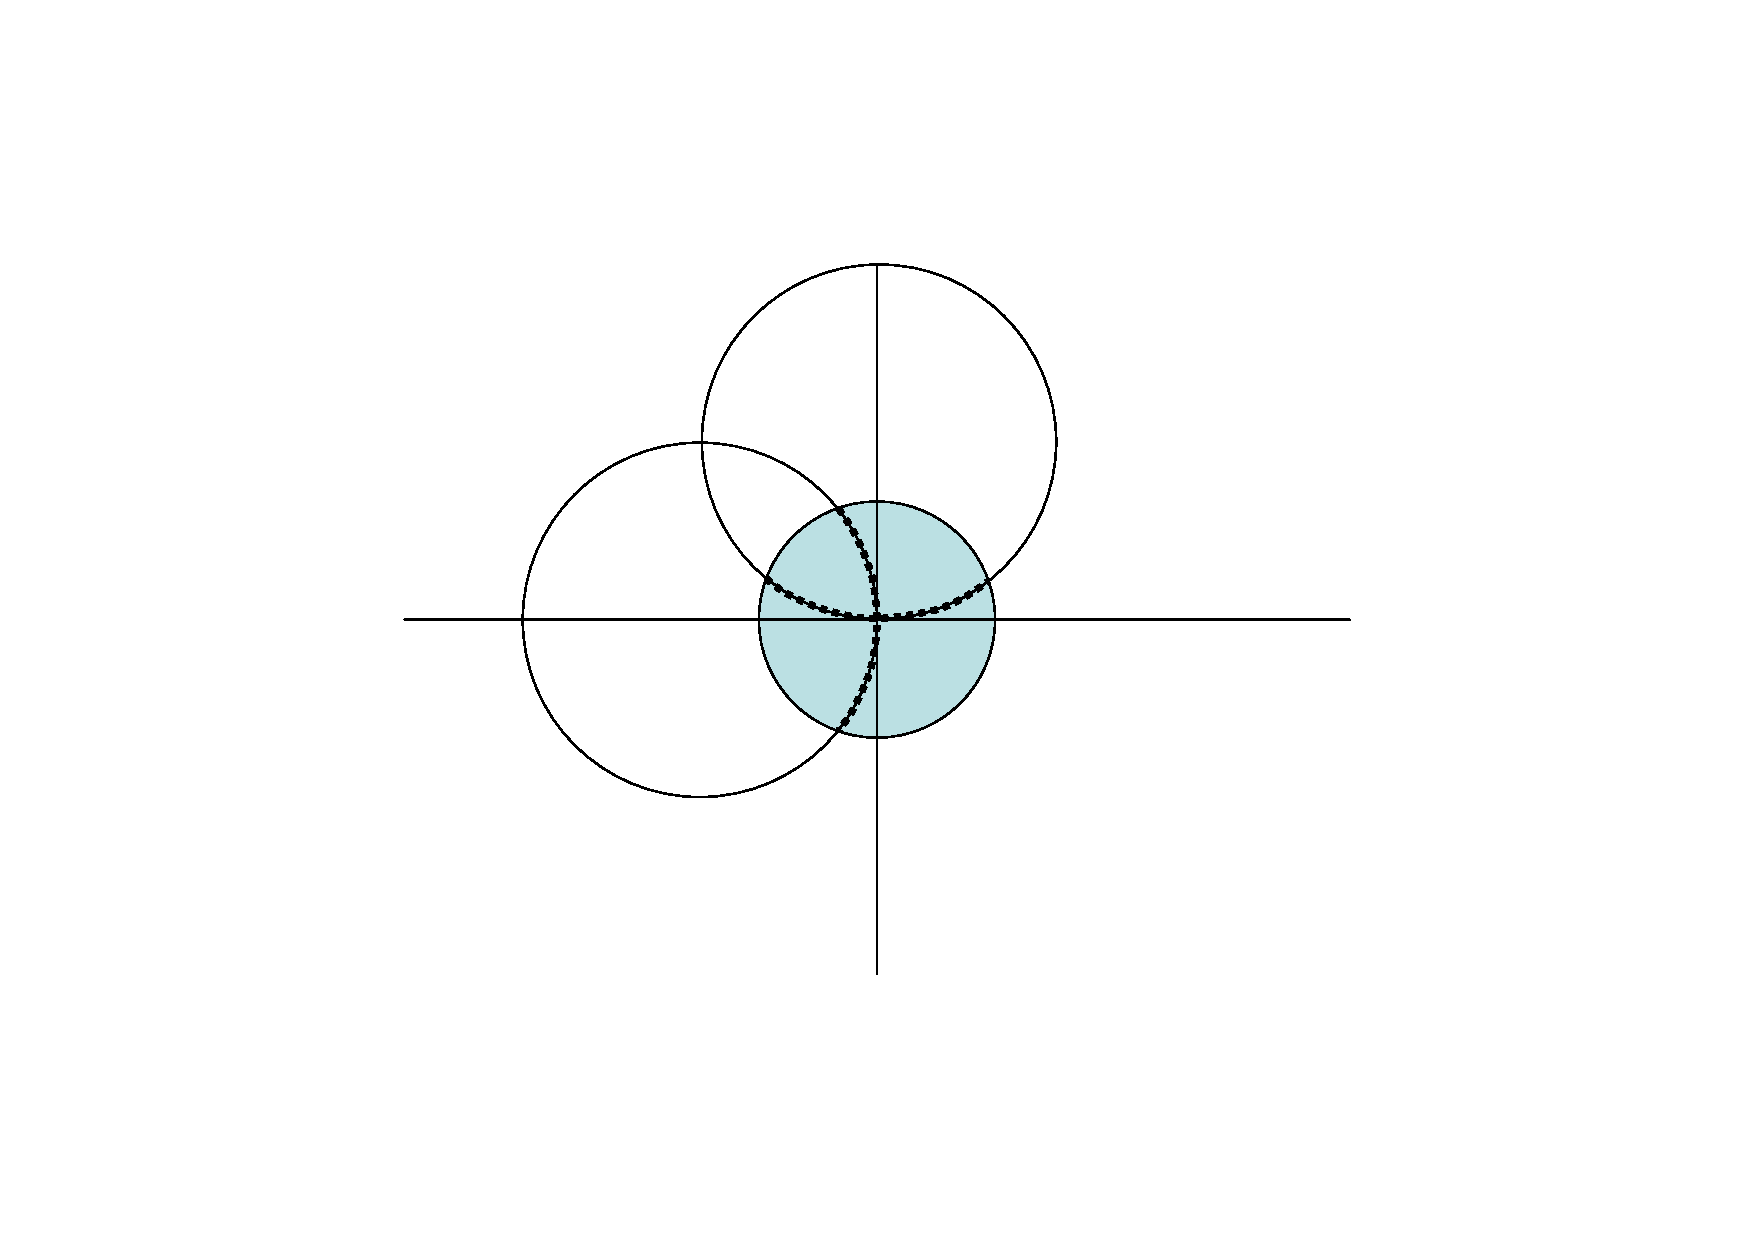
\includegraphics[scale=0.5]{figures/Ewald2Image.pdf}
\end{frame}

\begin{frame}
\frametitle{Indexing}
\hspace{6cm}
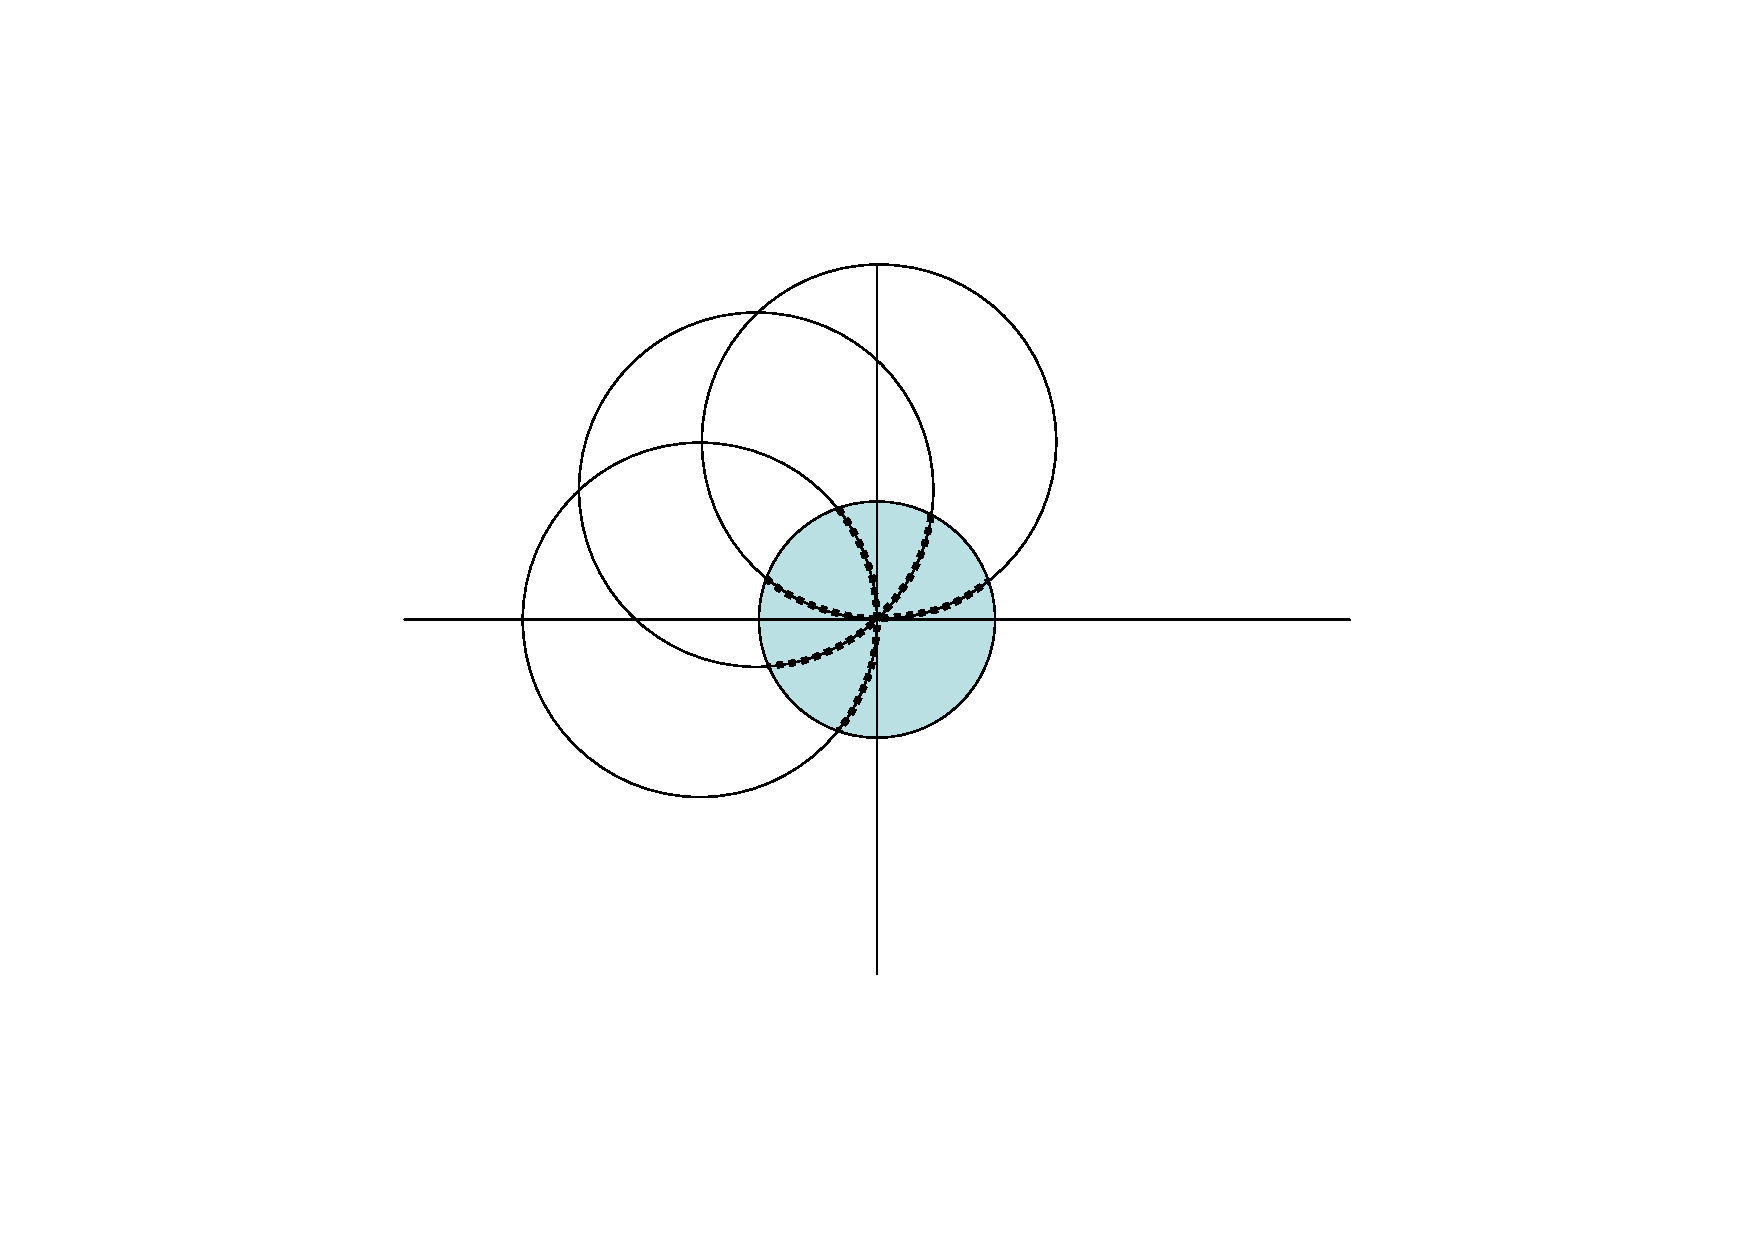
\includegraphics[scale=0.5]{figures/Ewald3Image.pdf}
\end{frame}

\begin{frame}
\frametitle{Scaling}
\hspace{2cm}
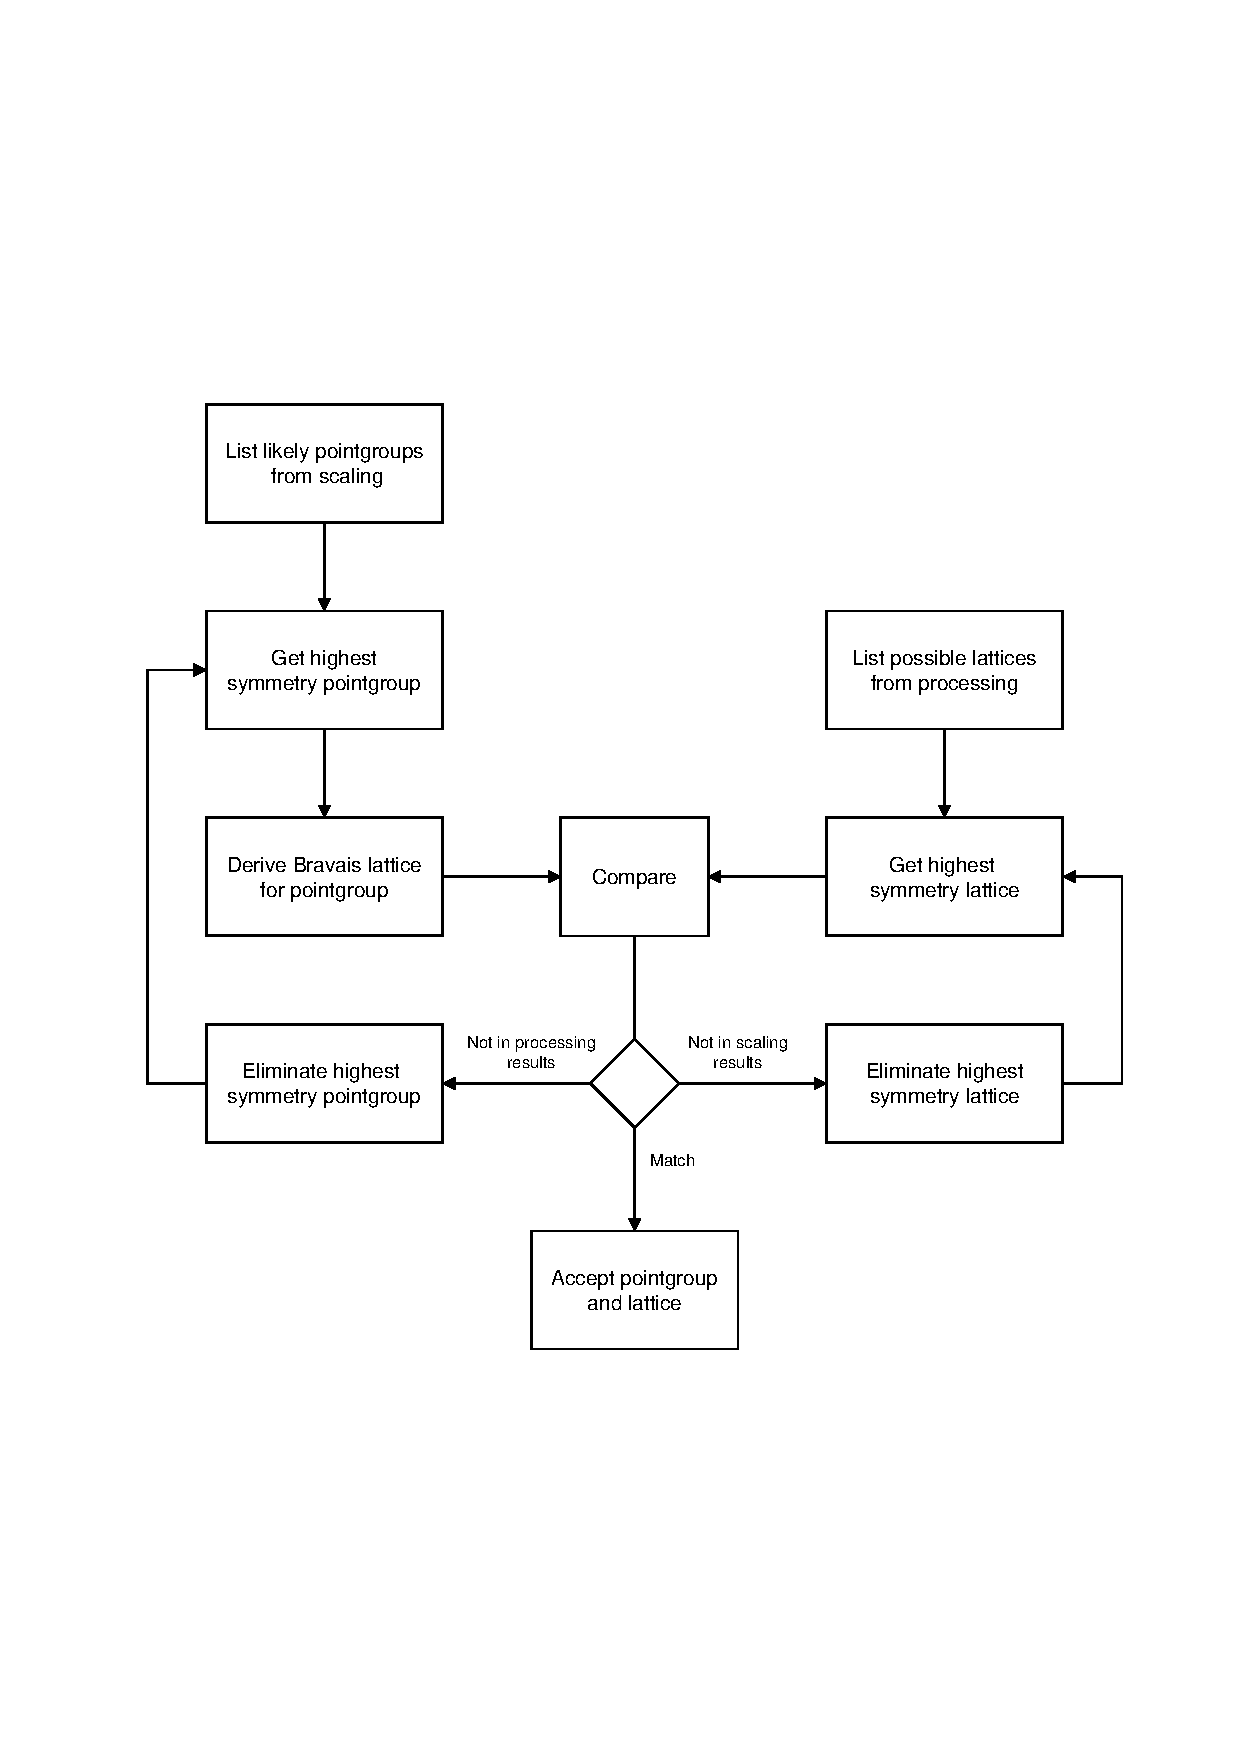
\includegraphics[scale=0.5]{figures/scaling-step-1.pdf}
\end{frame}

\begin{frame}
\frametitle{Scaling}
\hspace{2cm}
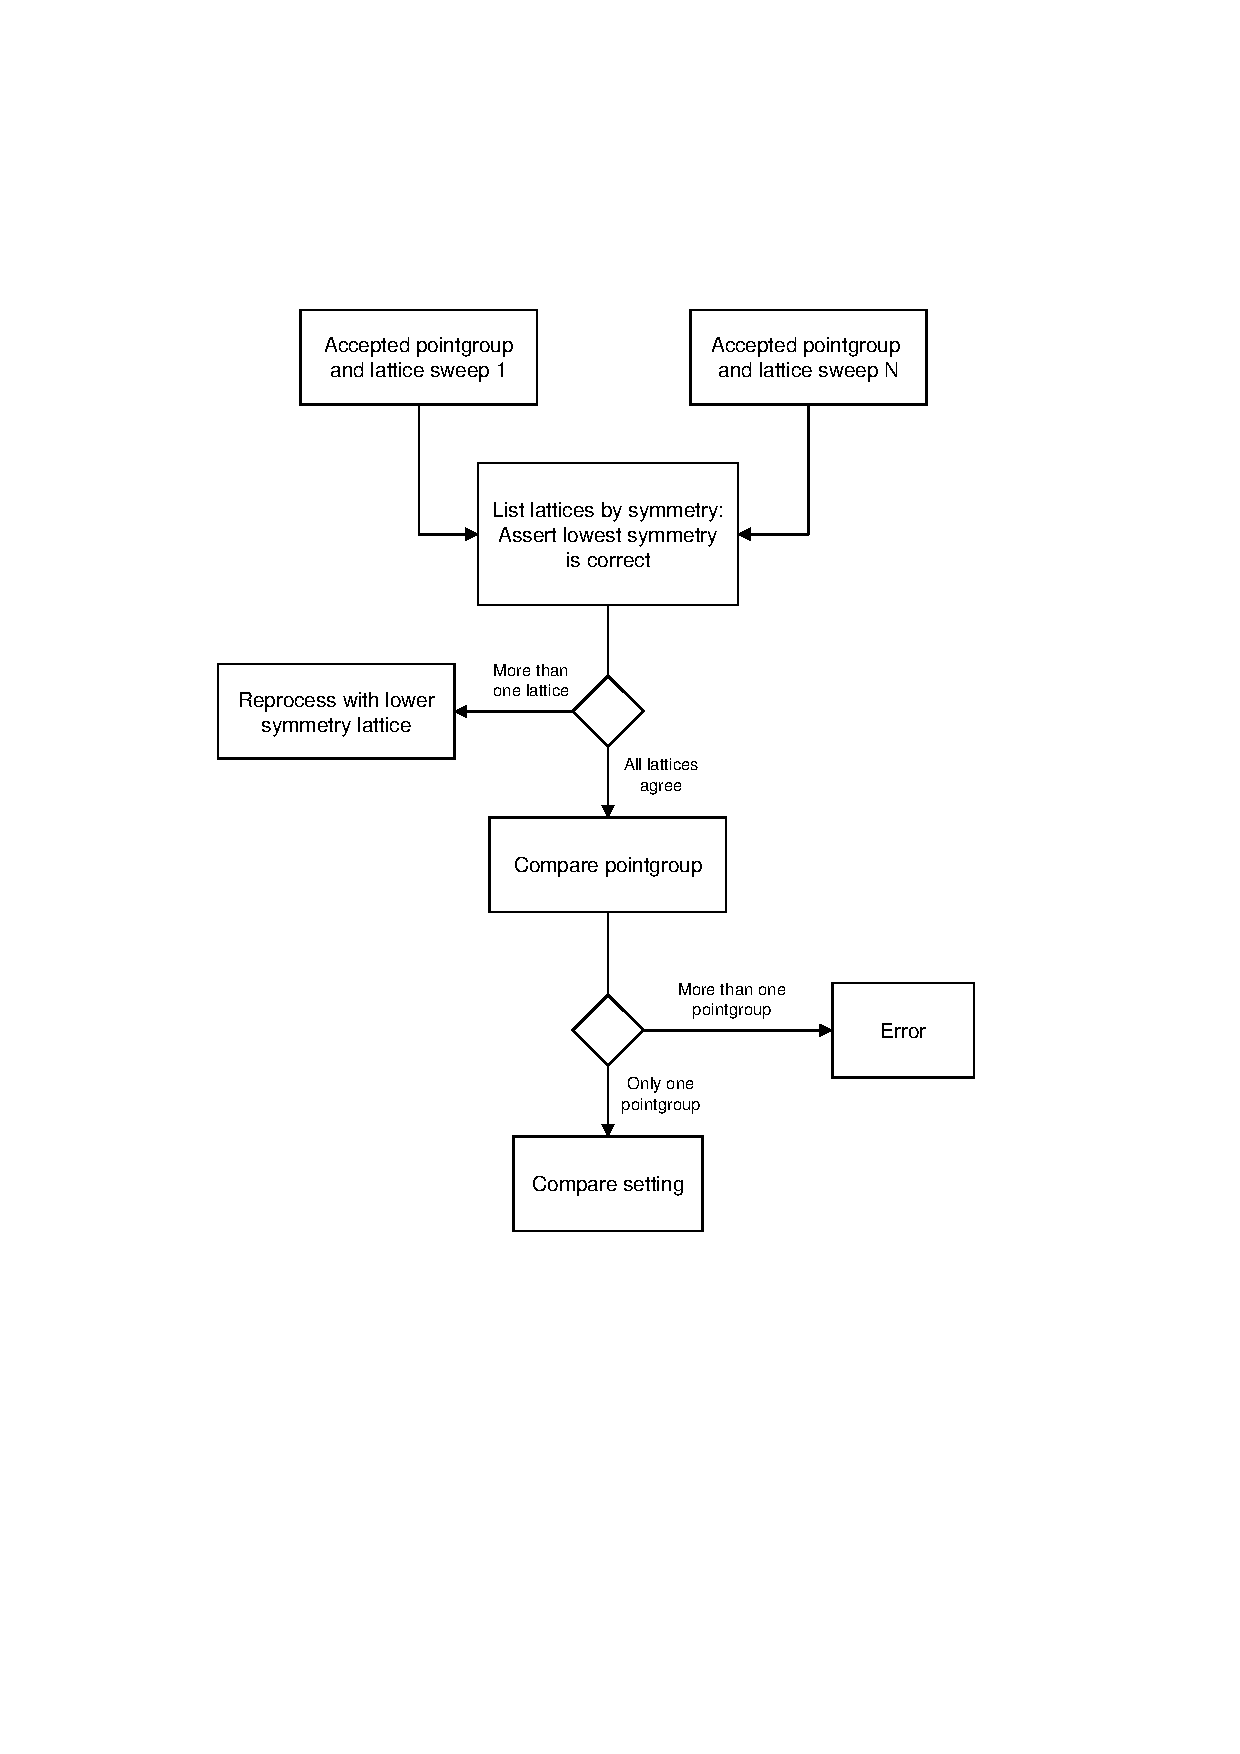
\includegraphics[scale=0.5]{figures/scaling-step-2.pdf}
\end{frame}

\begin{frame}
\frametitle{Scaling}
\hspace{2cm}
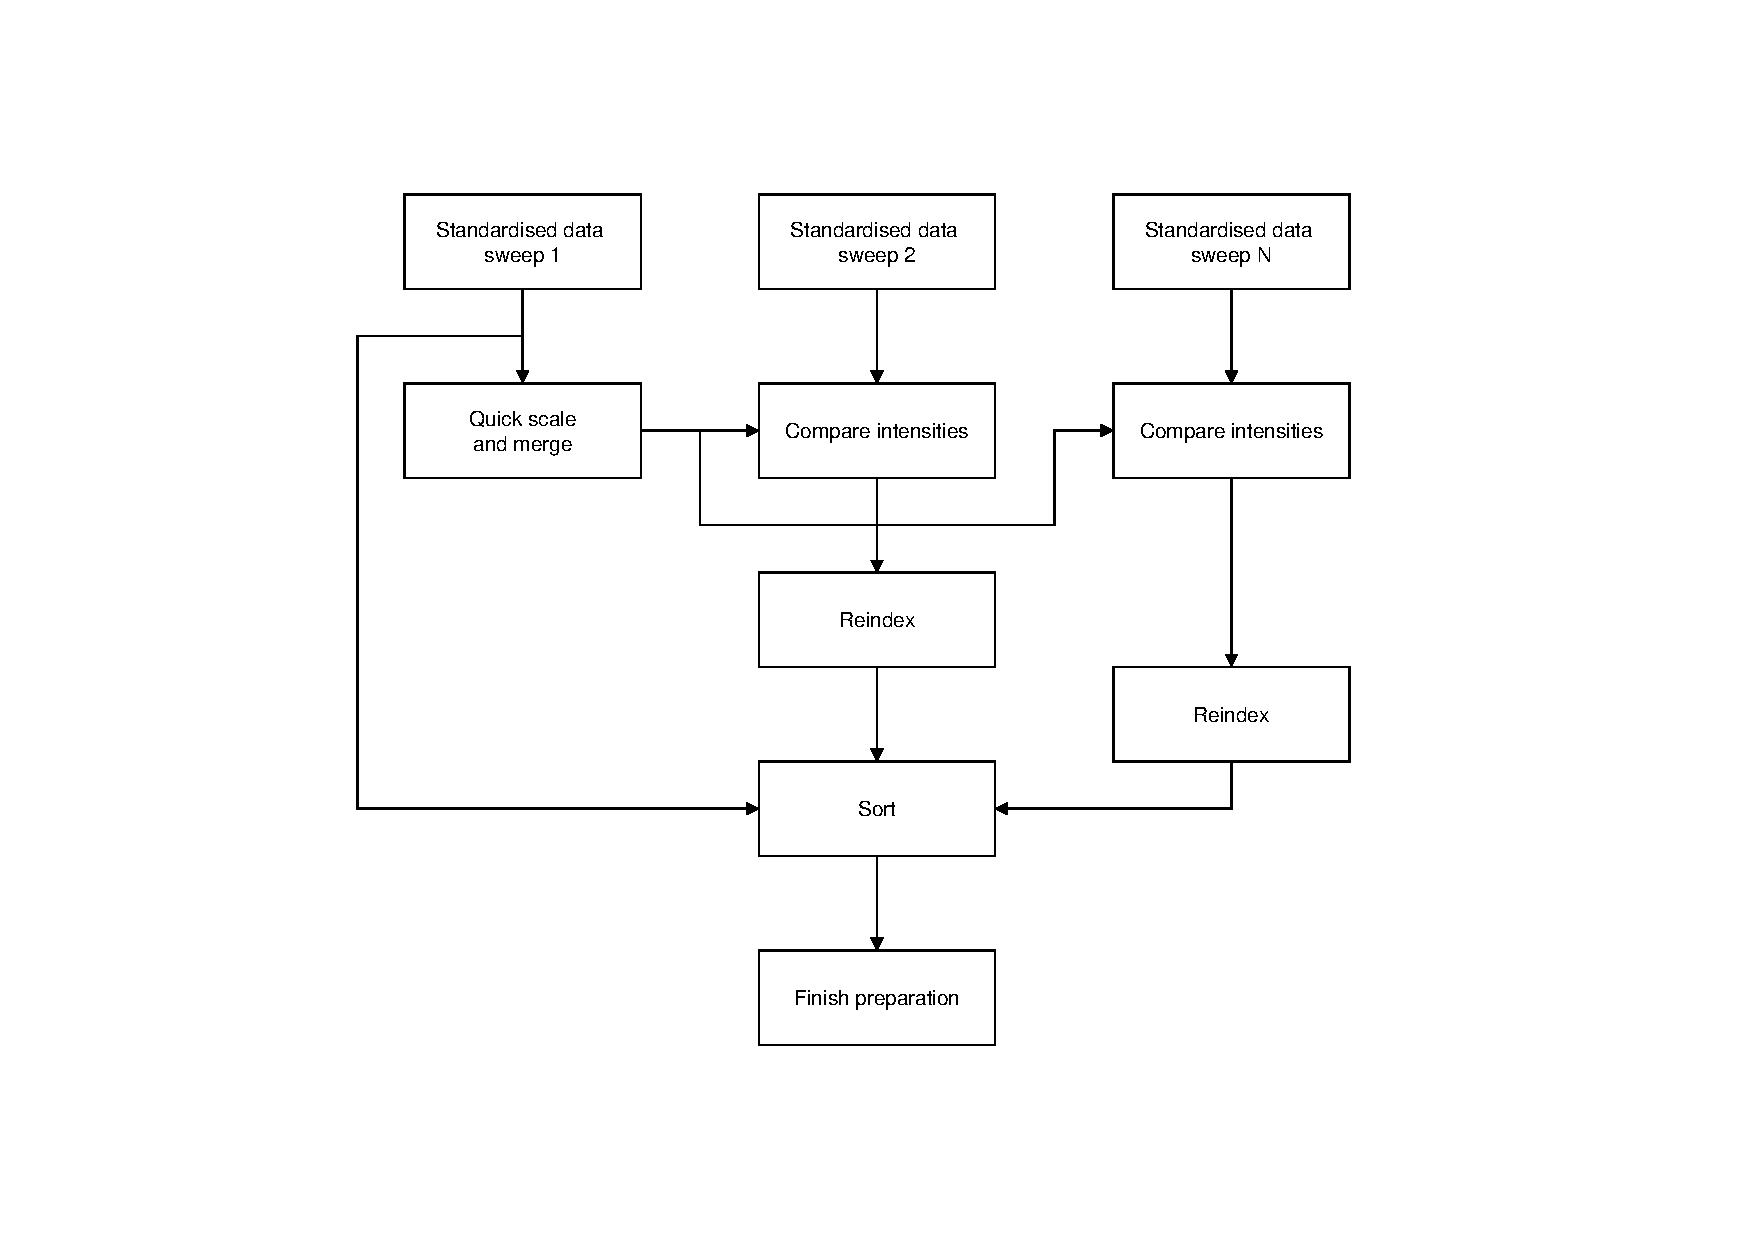
\includegraphics[scale=0.5]{figures/scaling-step-3.pdf}
\end{frame}

\end{document}
